\documentclass[12pt,a4paper]{article}
\usepackage[utf8]{inputenc}
\usepackage[brazil]{babel}
\usepackage{graphicx}
\usepackage{caption}
\usepackage{siunitx}
\usepackage{changepage}
\usepackage{setspace}
\usepackage{float}
\usepackage[a4paper]{geometry}
\usepackage{amsmath,amsfonts,amstext,amscd,bezier}
\usepackage{mathtools}
\usepackage{amsthm}
\usepackage{mathrsfs}
\usepackage{times}
\usepackage{indentfirst}
\usepackage{hyperref}
\usepackage{placeins}
\usepackage{array}
\usepackage{subfigure}
\usepackage{wrapfig}
\usepackage{setspace}
\usepackage{gensymb}
\usepackage{svg}
\usepackage[backend=bibtex,sorting=none]{biblatex}
\usepackage{verbatim}
\usepackage[autostyle]{csquotes}
\usepackage{minted}
\linespread{1.1}

\begin{document}
	\begin{titlepage}
		\begin{center}
			\large Universidade de São Paulo\\[0.2cm]
			\large Instituto de Física de São Carlos\\[7cm]
			\huge \textbf{Relatório 5 - IntroFisComp}\\[6cm]
			
			\large Alexandre de Taunay Voloch \\[0.2cm]
		\end{center}
	\end{titlepage}

\section{Tarefa 1}
\subsection{a}

Para que a órbita seja circular, precisamos que ela satisfaça a equação do movimento circular, isto é,

\[ a = \frac{v^2}{r} \]

Temos $F = ma$. Logo,

\[ a = \ddot{\rho} = \frac{1}{\rho^2} = \frac{v^2}{\rho} \]

Logo

\[ v_0 = \frac{1}{\sqrt{\rho_0}} \]

Como foi dado que $\rho_0 = (a, 0)$, a velocidade deve apontar apenas na direção $y$. Logo, $v_0 = (0, \frac{1}{\sqrt{a}})$.

\subsection{b}

Segue o programa:

\begin{minted}[
	mathescape,
	linenos,
	fontsize=\footnotesize,
	framesep=2mm,
	breaklines]
	{fortranfixed}
            implicit real*8 (a-h, o-z)
            real*8 p_ec(10000000,2)
            real*8 v_ec(10000000,2)
            real*8 p_verlet(10000000,2)
            real*8 v_verlet(10000000,2)

            pi = 4.d0*datan2(1.d0,1.d0)

            tau_total = 10d0
            dtau = 1d-4
            iteracoes = int(tau_total/dtau)
            a = 1d0

            open(file='tarefa-1-saida-pec.dat', unit=1)
            open(file='tarefa-1-saida-pverlet.dat', unit=3)
            open(file='tarefa-1-saida-vec.dat', unit=2)
            open(file='tarefa-1-saida-verlet.dat', unit=4)

            p_ec(1,1) = a
            p_ec(1,2) = 0d0
            v_ec(1,1) = 0d0
            v_ec(1,2) = 1d0/dsqrt(a)

            p_verlet(1,1) = a
            p_verlet(1,2) = 0d0

            do i=2,iteracoes
               p3 = pcubo(p_ec(i-1,1), p_ec(i-1,2))

               v_ec(i,1) = v_ec(i-1,1) - (p_ec(i-1,1)/p3)*dtau
               v_ec(i,2) = v_ec(i-1,2) - (p_ec(i-1,2)/p3)*dtau

               p_ec(i,1) = p_ec(i-1,1) + v_ec(i,1)*dtau
               p_ec(i,2) = p_ec(i-1,2) + v_ec(i,2)*dtau

               write(1,*)p_ec(i,1),p_ec(i,2)
               write(2,*)v_ec(i,1),v_ec(i,2)

               !verlet
               if (i.eq.2) then
                  ! pular verlet, usar os valores de euler-cromer
                  p_verlet(i,1) = p_ec(i,1)
                  p_verlet(i,2) = p_ec(i,2)
               else
                  p3 = pcubo(p_verlet(i-1,1),p_verlet(i-1,2))

                  p_verlet(i,1) = 2d0*p_verlet(i-1,1) - p_verlet(i-2,1)
     &            - (p_verlet(i-1,1)/p3)*(dtau**2)
                  p_verlet(i,2) = 2d0*p_verlet(i-1,2) - p_verlet(i-2,2)
     &            - (p_verlet(i-1,2)/p3)*(dtau**2)
               endif

               write(3,*)p_verlet(i,1), p_verlet(i,2)

            end do

            ! agora calcular as velocidades em Verlet
            ! vamos usar a derivdada simétrica de 5 pontos
            do i=3,iteracoes-2
               ! começamos do 3 pq precisamos ter i-2 e i-1 válidos
               v_verlet(i,1) = (p_verlet(i-2,1) - 8d0*p_verlet(i-1,1)
     &         + 8d0*p_verlet(i+1,1) - p_verlet(i+2,1)) / (12d0*dtau)
               v_verlet(i,2) = (p_verlet(i-2,2) - 8d0*p_verlet(i-1,2)
     &         + 8d0*p_verlet(i+1,2) - p_verlet(i+2,2)) / (12d0*dtau)

               write(4,*)v_verlet(i,1), v_verlet(i,2)
            end do

            end

            function pcubo(px,py)
               real*8 px, py, pcubo
               pcubo = (px**2d0 + py**2d0)**(3d0/2d0)
            end function

\end{minted}

Simulando a órbita da terra (isto é, com $\rho_0 = 1 = v_0$) temos

\begin{figure}[H]
\centering
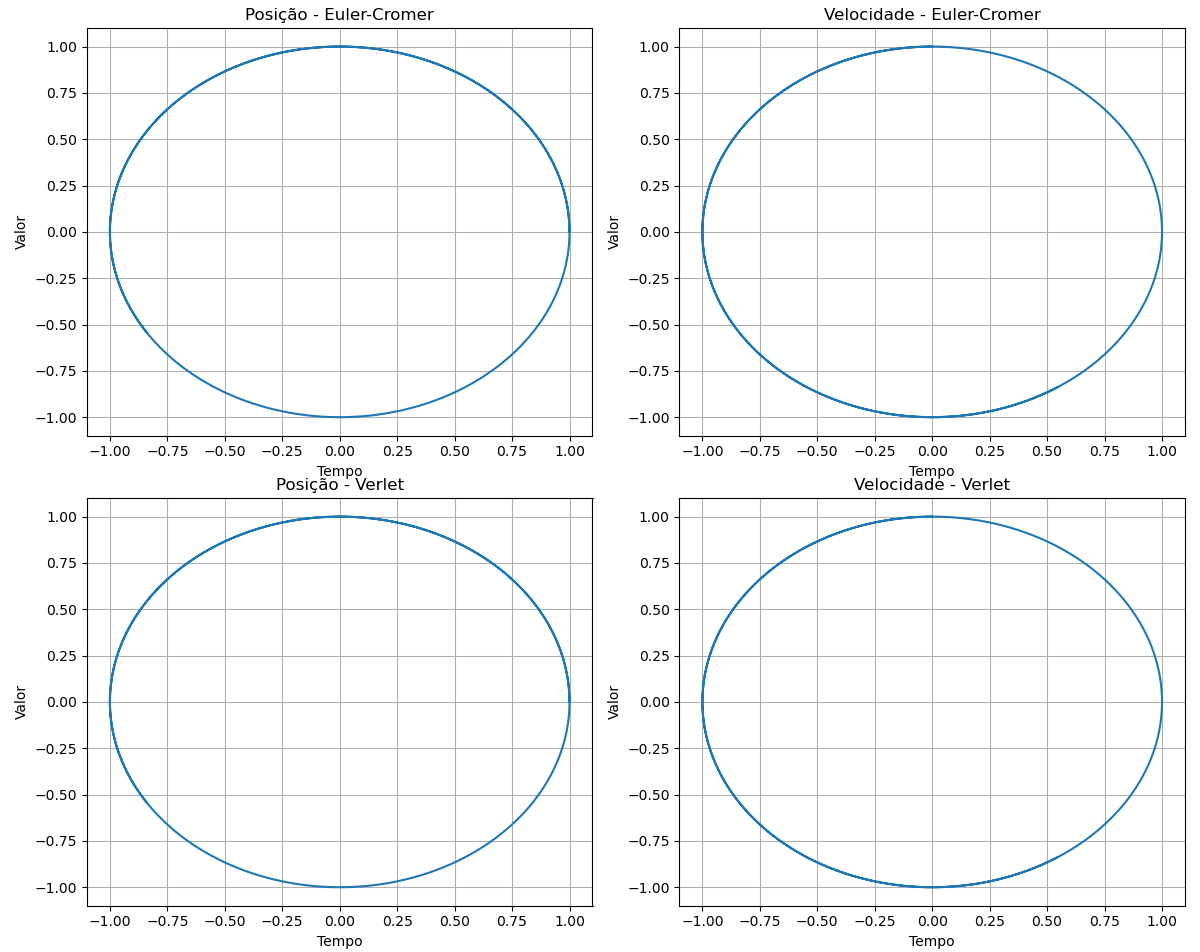
\includegraphics[width=\linewidth]{../tarefa-1b/graficos.png}
\caption{Gráfico da órbita da terra e velocidade calculada nos diferentes métodos.}
\end{figure}

Como podemos ver, todos os gráficos são praticamente idênticos. Isso é de se esperar, pois a velocidade e a posição têm o mesmo módulo a todo momento, e por ser movimento circular vão apenas oscilando em um círculo, embora com fases diferentes (caso fizéssemos uma animação, veríamos isso).

\subsection{c}
Aqui usamos o seguinte programa para fazer os gráficos:

\begin{minted}[
	mathescape,
	linenos,
	fontsize=\footnotesize,
	framesep=2mm,
	breaklines]
	{fortranfixed}
      implicit real*8 (a-h, o-z)
      real*8 p_ec(10000000,2)
      real*8 v_ec(10000000,2)
      real*8 p_verlet(10000000,2)
      real*8 v_verlet(10000000,2)
      real*8 m_planetas(8), a_planetas(8)
      real*8 d_planetas(800,100000,2) ! armazena (dtau, delta) respectivo pra aquele planeta
      data m_planetas / 0.055d0, 0.817d0, 1.00d0, 0.107d0,
     &318d0, 95.2d0, 14.5d0, 17.1d0 /
      data a_planetas / 0.39d0, 0.72d0, 1.00d0, 1.52d0,
     &5.20d0, 9.58d0, 19.2d0, 30.1d0/
!      data a_planetas / 0.39d0, 0.72d0, 1.00d0, 1.52d0,
!     &5.20d0, 6.58d0, 8.2d0, 9.0d0/

      pi = 4.d0*datan2(1.d0,1.d0)

      open(file='tarefa-1c-saida-dec.dat', unit=1)
      open(file='tarefa-1c-saida-dverlet.dat', unit=2)
      open(file='dtaumax.dat', unit=3)

      ! iterar nos planetas
      !do ip=5,60
      do ip=3,4
         !a = dble(ip)*0.1d0*a_planetas(3)
         write(*,*)"Planeta",ip,"a",a
         a = a_planetas(ip)

         p_ec(1,1) = a
         p_ec(1,2) = 0d0
         v_ec(1,1) = 0d0
         v_ec(1,2) = 1d0/dsqrt(a)

         p_verlet(1,1) = a
         p_verlet(1,2) = 0d0

         iquanto=20

         iter_dtau = int(3.5*iquanto)

         !tau_total = 50d0
         tau_total = 20d0*a

         do j=1,iter_dtau
            potencia = dble(2*iquanto +j)/dble(iquanto)
            dtau = 10**(-potencia)
            iteracoes = int(tau_total/dtau)

            write(*,*)"dtau",dtau,j
            pmax_ec = 0d0
            pmin_ec = 10000000d0
            pmax_v = 0d0
            pmin_v = 10000000d0

            do i=2,iteracoes
               p3 = pcubo(p_ec(i-1,1), p_ec(i-1,2))

               v_ec(i,1) = v_ec(i-1,1) - (p_ec(i-1,1)/p3)*dtau
               v_ec(i,2) = v_ec(i-1,2) - (p_ec(i-1,2)/p3)*dtau

               p_ec(i,1) = p_ec(i-1,1) + v_ec(i,1)*dtau
               p_ec(i,2) = p_ec(i-1,2) + v_ec(i,2)*dtau

               !verlet
               if (i.eq.2) then
                  ! pular verlet, usar os valores de euler-cromer
                  p_verlet(i,1) = p_ec(i,1)
                  p_verlet(i,2) = p_ec(i,2)
               else
                  p3 = pcubo(p_verlet(i-1,1),p_verlet(i-1,2))

               p_verlet(i,1) = 2d0*p_verlet(i-1,1) - p_verlet(i-2,1)
     &          - (p_verlet(i-1,1)/p3)*(dtau**2)
               p_verlet(i,2) = 2d0*p_verlet(i-1,2) - p_verlet(i-2,2)
     &          - (p_verlet(i-1,2)/p3)*(dtau**2)
               endif

               ! calcular p
            p_modulo_ec = dsqrt(p_ec(i,1)**2d0 + p_ec(i,2)**2d0)
            p_modulo_v = dsqrt(p_verlet(i,1)**2d0 + p_verlet(i,2)**2d0)

               if (p_modulo_ec.gt.pmax_ec) then
                  pmax_ec = p_modulo_ec
               else if (p_modulo_ec.lt.pmin_ec) then
                  pmin_ec = p_modulo_ec
               end if
               if (p_modulo_v.gt.pmax_v) then
                  pmax_v = p_modulo_v
               else if (p_modulo_v.lt.pmin_v) then
                  pmin_v = p_modulo_v

               endif


            end do

            !write(*,*)"Pmax e min:", pmax_ec,pmin_ec,pmax_v,pmin_v

            d_ec = pmax_ec/pmin_ec - 1
            d_v = pmax_v/pmin_v - 1


            ! escrever no grafico valores p/ terra

            if (ip.eq.3)then
               write(1,*)potencia,d_ec
               write(2,*)potencia,d_v
            endif

            d_planetas(ip,j,1) = dtau
            d_planetas(ip,j,2) = d_ec

            write(*,*)"d ec:",d_ec,"d verlet:",d_v

            !if(d_ec.lt.1d-3)then
            !   goto 20
            !endif

         end do
20         continue
      end do

      ! agora processar os dados de d_planetas para fazer o gráfico de dtau_min x a
      write(*,*)"processando"
      !do ip=5,60
      !   write(*,*)"planeta",ip
      !   do j=1,iter_dtau
      !      if(d_planetas(ip,j,2).le.1d-3)then
      !         write(*,*)"saimos"
      !         goto 10
      !      endif
      !   end do
!10    !   write(3,*)dble(ip)*0.1d0*a_planetas(3),d_planetas(ip,j,1),j

      !end do

      end

      function pcubo(px,py)
         real*8 px, py, pcubo
         pcubo = (px**2d0 + py**2d0)**(3d0/2d0)
      end function

\end{minted}

Primeiro, fazemos o gráfico de $\delta$ em função de $\Delta\tau$. Obtemos o seguinte:

\begin{figure}[H]
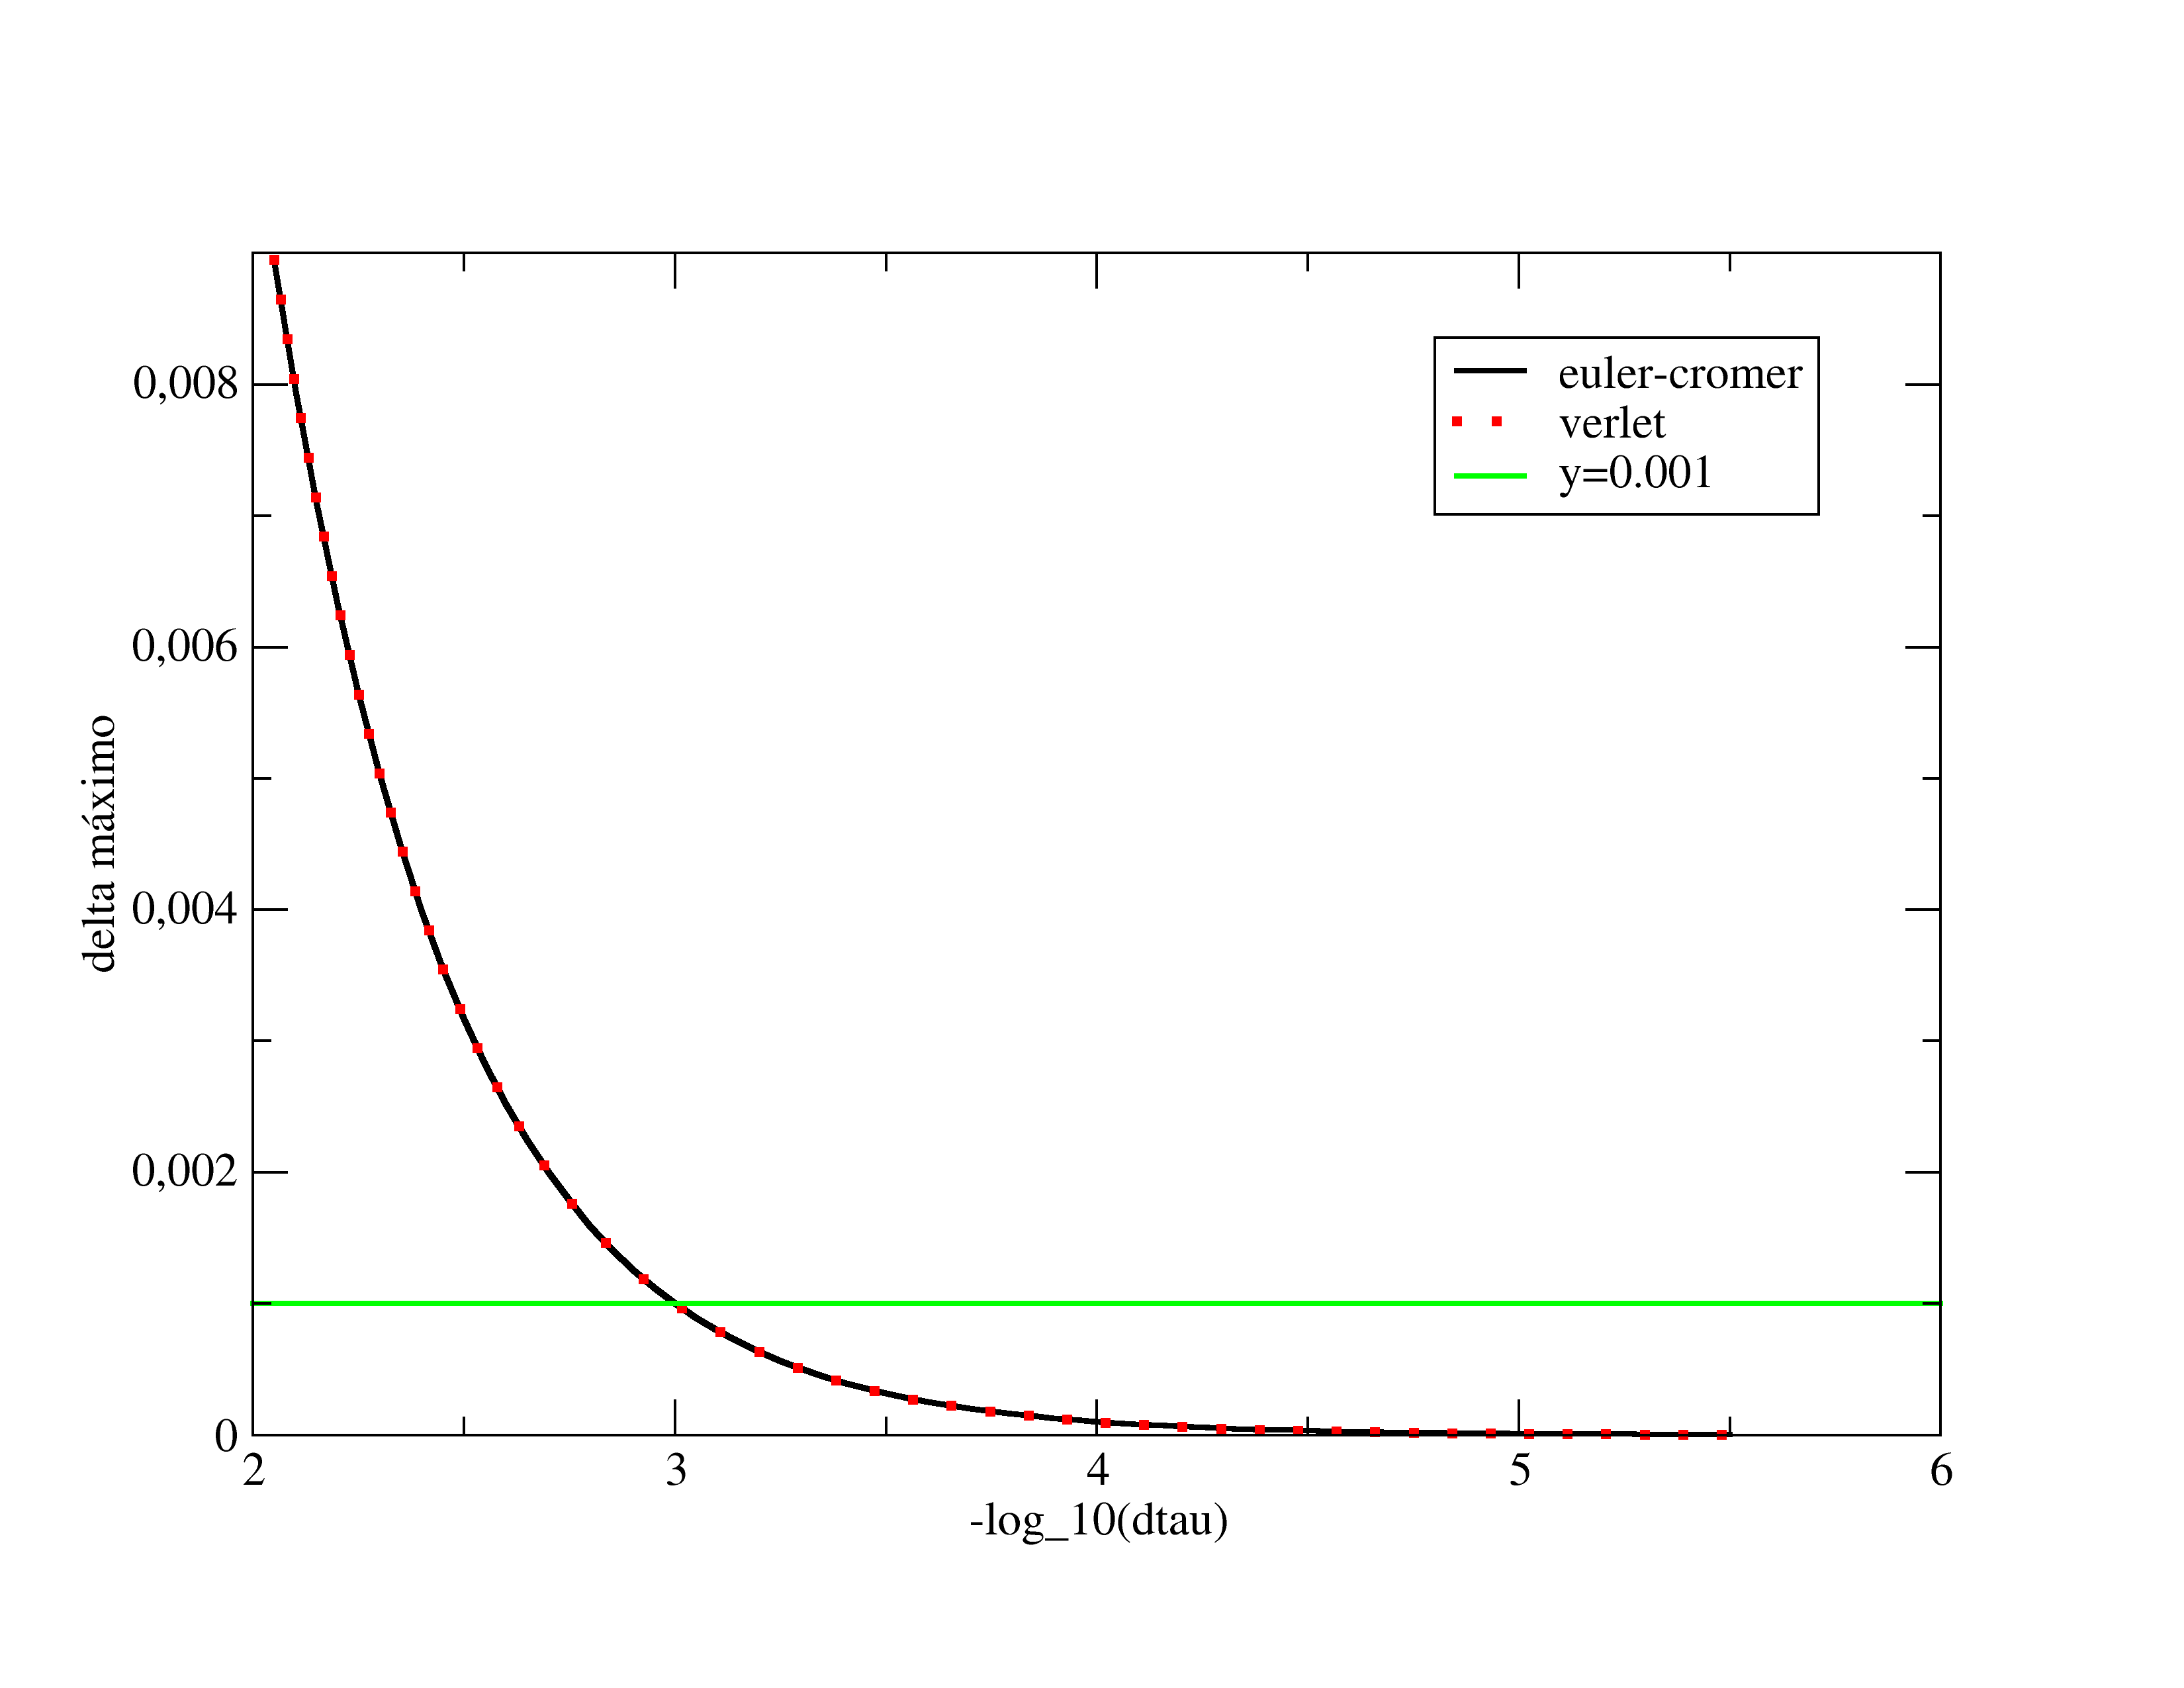
\includegraphics[width=\linewidth]{../tarefa-1c/grafico_deltas.png}
\caption{Gráfico de $\delta$ em função de $\Delta\tau$, para a órbita da Terra}
\end{figure}

Verificamos que, para a órbita da Terra em específico, o delta máximo é praticamente igual ao $\Delta\tau$. Portanto, se queremos $\delta < 10^{-3}$, este também deve ser o valor de $\Delta\tau$.

Agora, fazendo o gráfico para diversos raios diferentes (para isso simulamos vários planetas no nosso programa), obtemos o seguinte:

\begin{figure}[H]
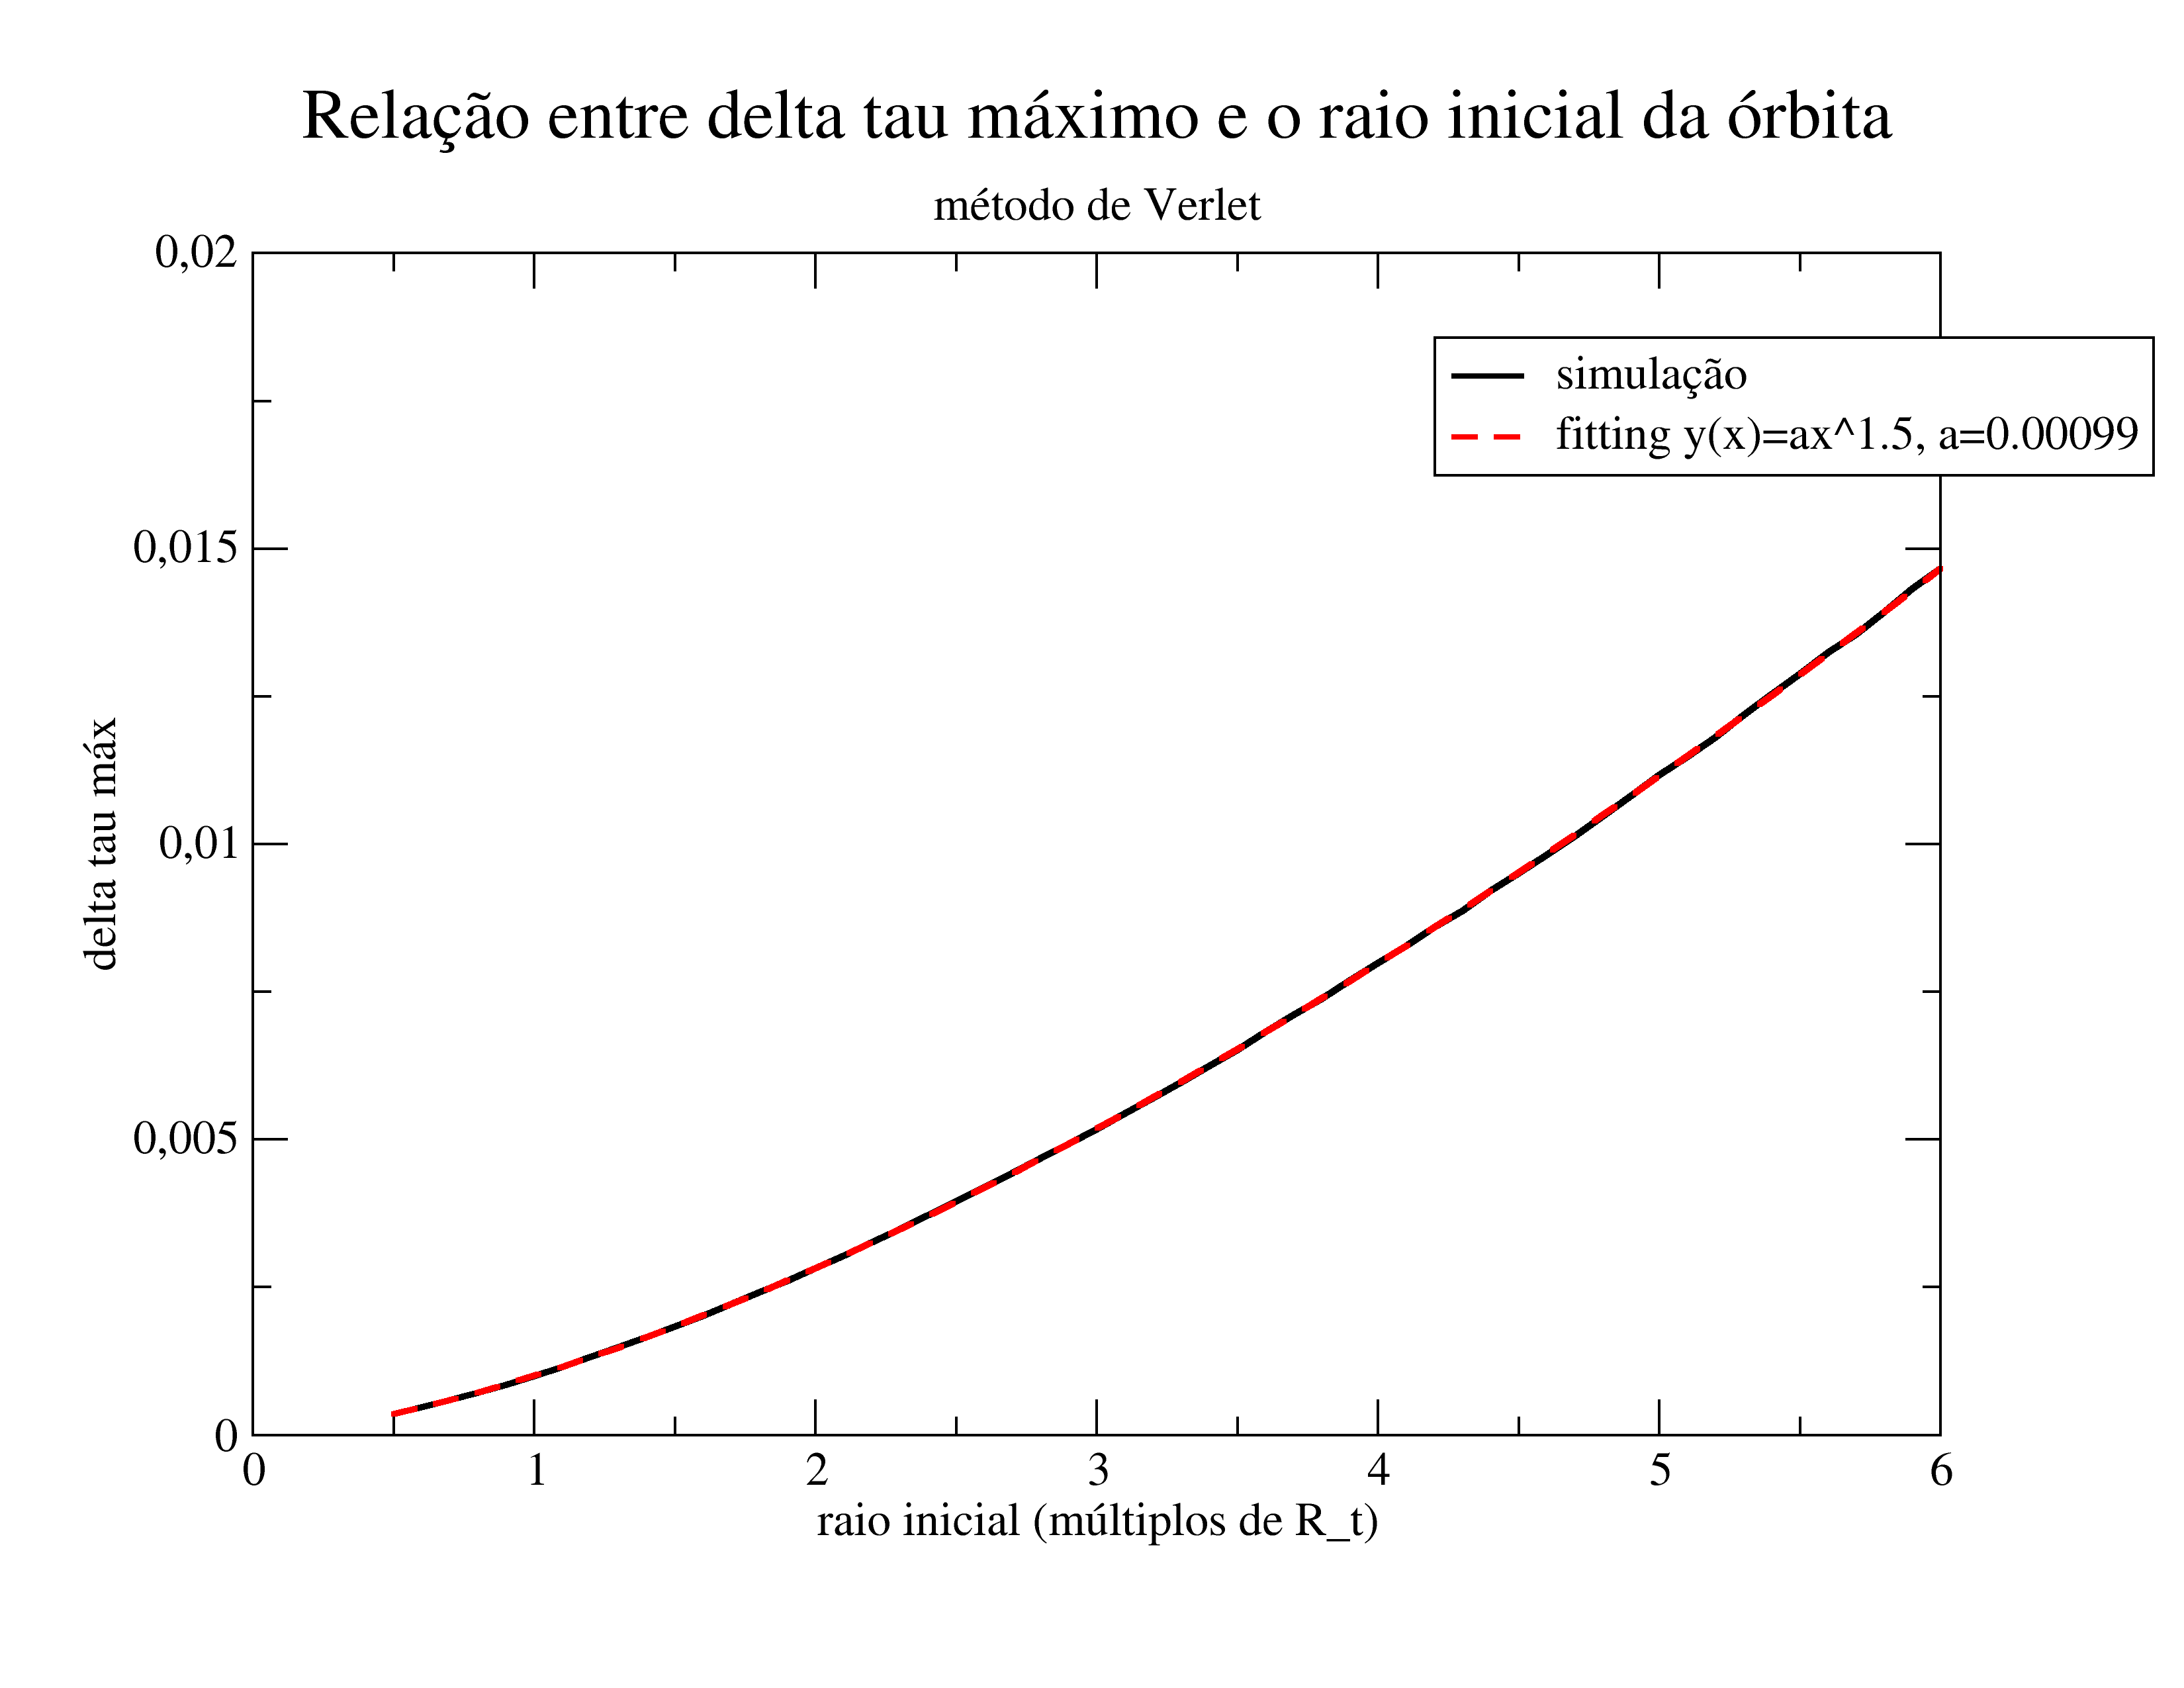
\includegraphics[width=\linewidth]{../tarefa-1c/grafico_dtaumax_bom_verlet.png}
\caption{Gráfico de $\Delta\tau_{max}$ em função do raio inicial da órbita - Verlet}
\end{figure}

\begin{figure}[H]
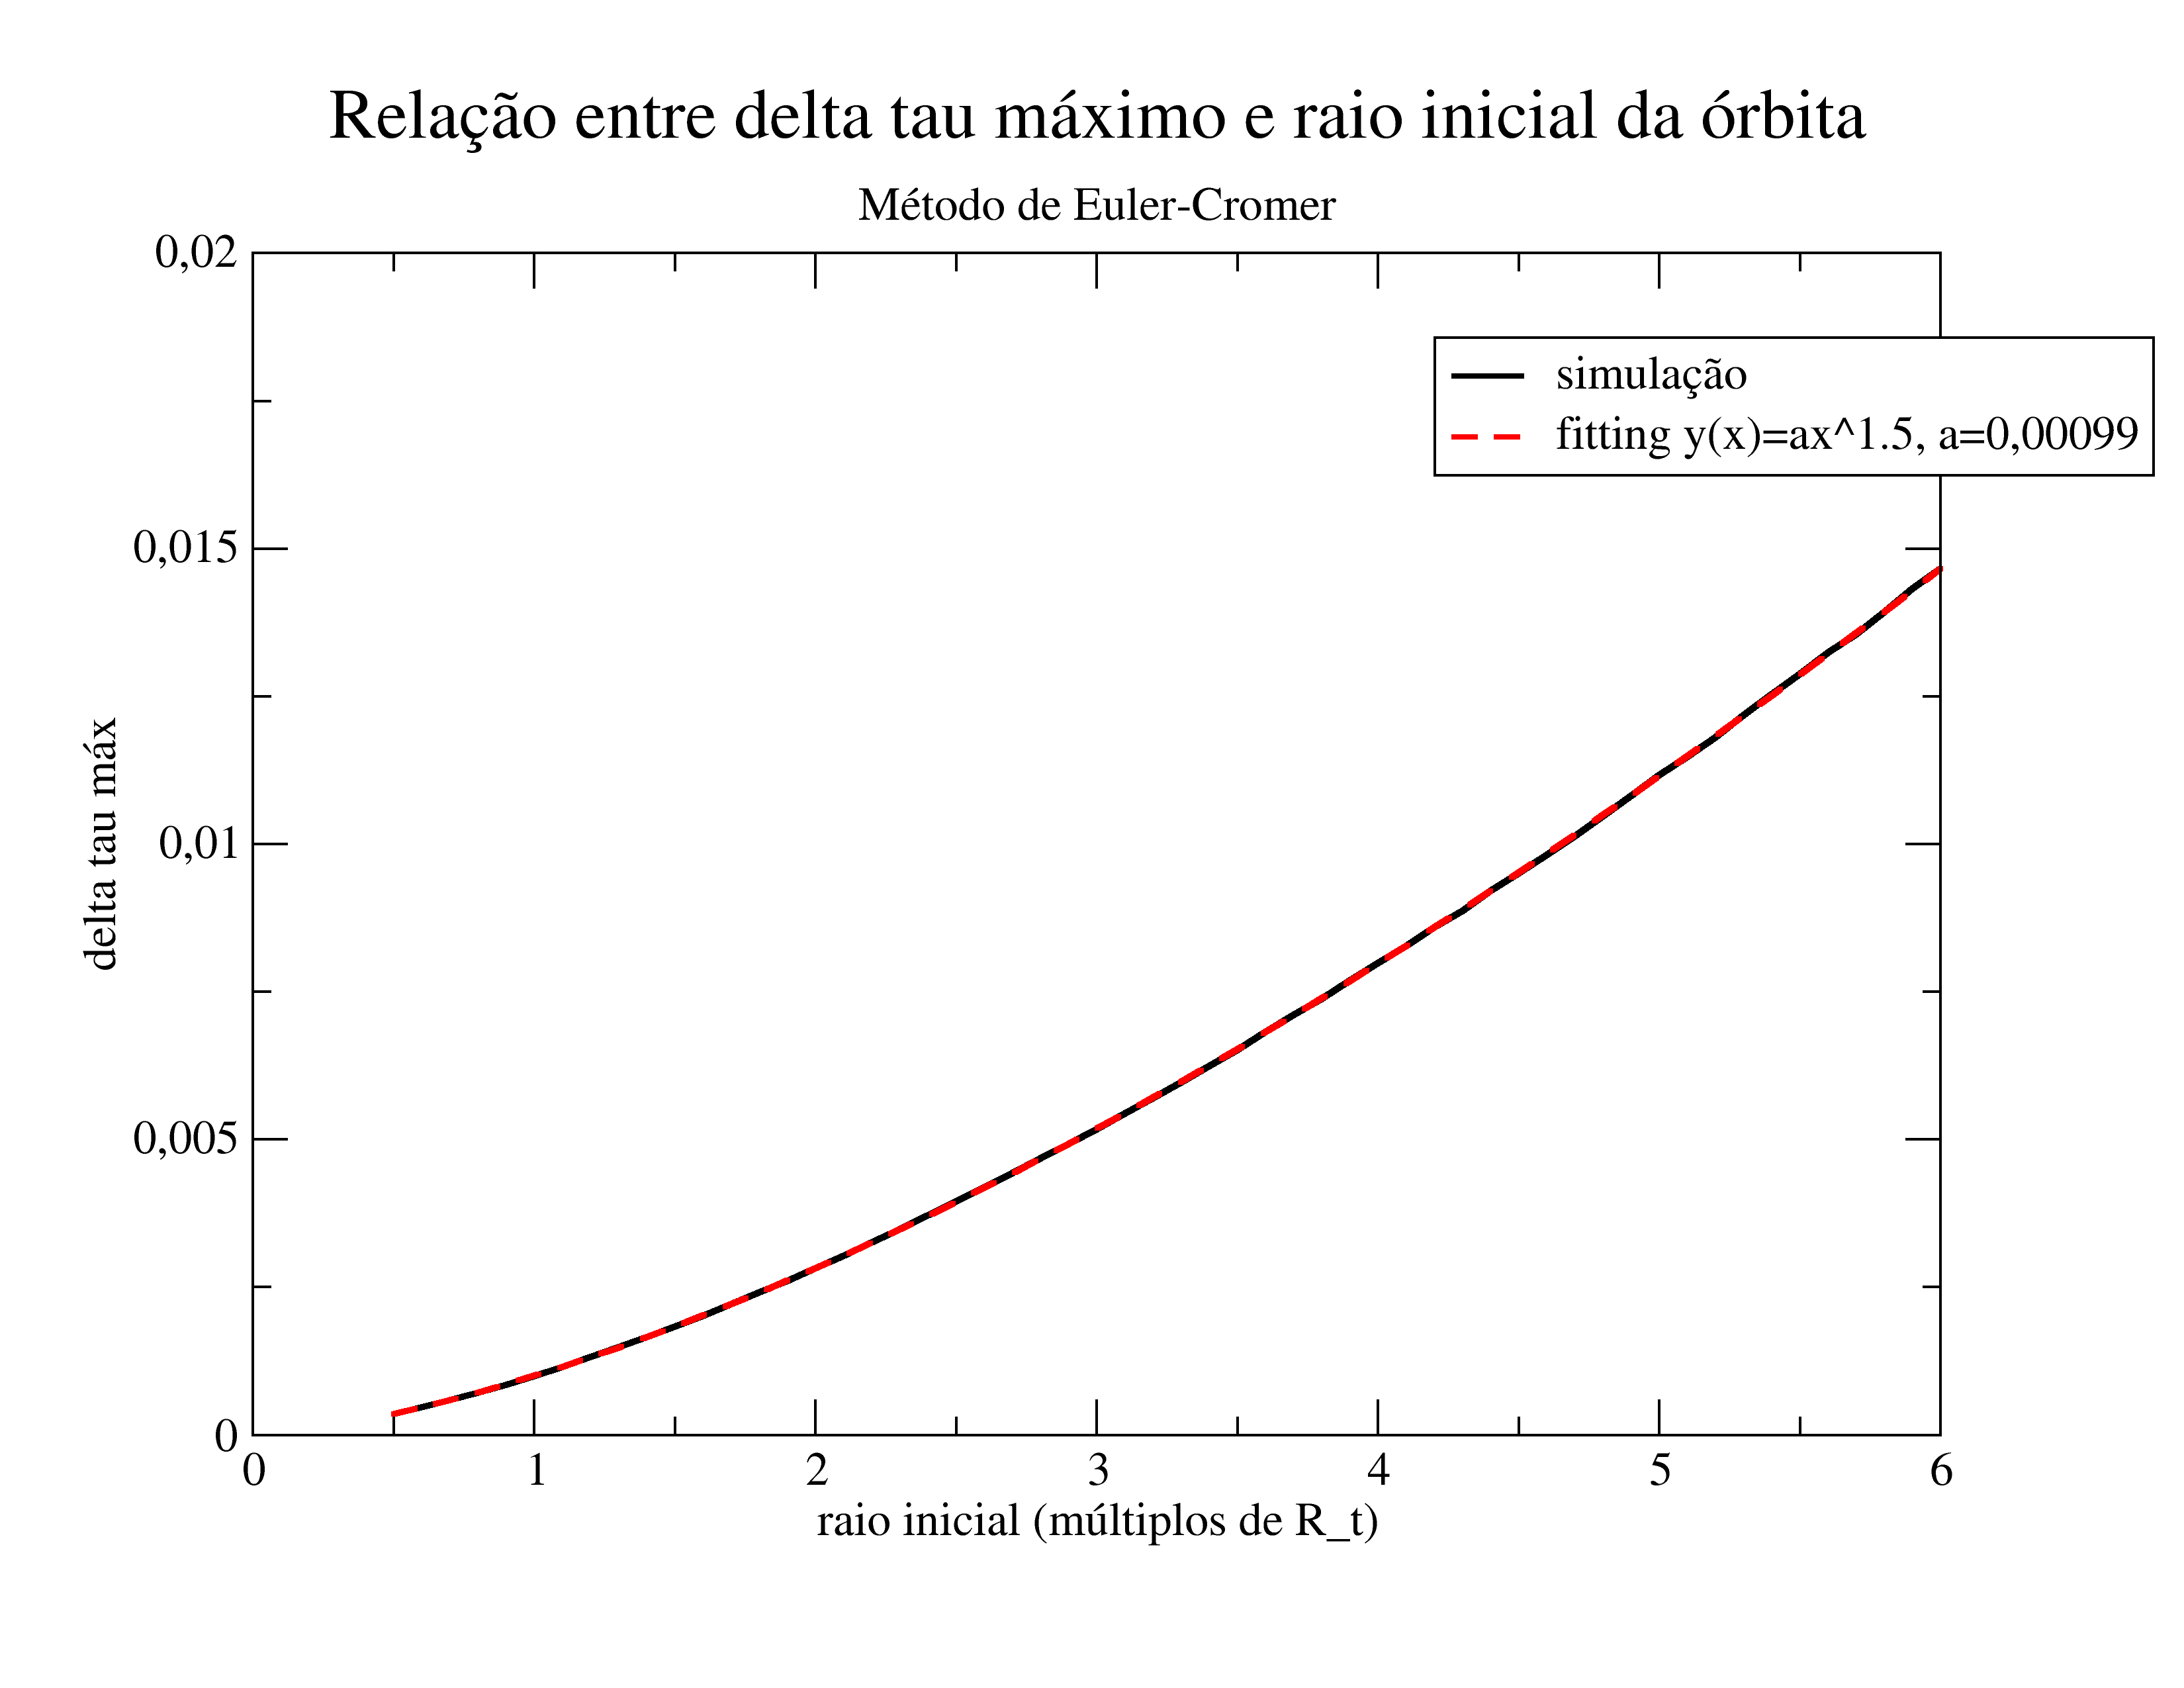
\includegraphics[width=\linewidth]{../tarefa-1c/grafico_dtaumax_ec.png}
\caption{Gráfico de $\Delta\tau_{max}$ em função do raio inicial da órbita - Euler-Cromer}
\end{figure}

Ambas as figuras são praticamente idênticas. Percebemos que a curva é fitada perfeitamente por uma função que é proporcional a $a^{3/2}$, o que confirma a hipótese feita no projeto.

Para explicar o motivo dessa proporcionalidade, precisamos assumir que $\Delta\tau_{max} \propto T$, onde $T$ nesse caso representa o período de órbita (em unidades de $\tau$). Assim, como a 3a lei de Kepler nos diz que $T \propto a^{3/2}$, a proporcionalidade também valerá para qualquer coisa proporcional a $T$.

\subsection{d}
Aqui utilizamos um programa muito parecido aos anteriores, mas que calcula a energia. Para chegar na expressão da energia adimensional, fazemos:

\[ E = \frac{m\dot{r}}{2} + \frac{GM_sm}{r} \]
\[ = \frac{m}{2}\frac{dr}{dt} + \frac{GM_sm}{r} 
= \frac{m}{2}\left( \frac{UAd\rho}{\frac{ano}{2\pi}d\tau}\right) ^2 + \frac{GM_sm}{UA\rho}
\]
\[ = \frac{4\pi^2m(UA)^2\dot{\rho}^2}{(ano)^2} + \frac{GM_sm}{UA\rho} \]
\[ = \frac{GM_sm}{UA}\left( \frac{\dot{\rho}^2}{2} + \frac{1}{\rho} \right)  \]

Logo, temos nossa expressão para energia adimensional:

\[ \epsilon = \frac{\dot{\rho}^2}{2} + \frac{1}{\rho} \]

\begin{minted}[
	mathescape,
	linenos,
	fontsize=\footnotesize,
	framesep=2mm,
	breaklines]
	{fortranfixed}
            implicit real*8 (a-h, o-z)
            real*8 p_ec(10000000,2)
            real*8 v_ec(10000000,2)
            real*8 p_verlet(10000000,2)
            real*8 v_verlet(10000000,2)

            pi = 4.d0*datan2(1.d0,1.d0)

            tau_total = 200d0
            dtau = 1d-3
            iteracoes = int(tau_total/dtau)
            a = 1d0

            open(file='energia-ec.dat',unit=1)
            open(file='energia-v.dat',unit=2)

            p_ec(1,1) = a
            p_ec(1,2) = 0d0
            v_ec(1,1) = 0d0
            v_ec(1,2) = 1d0/dsqrt(a)

            p_verlet(1,1) = a
            p_verlet(1,2) = 0d0

            do i=2,iteracoes
               tempo = dble(i)*dtau
               p3 = pcubo(p_ec(i-1,1), p_ec(i-1,2))

               v_ec(i,1) = v_ec(i-1,1) - (p_ec(i-1,1)/p3)*dtau
               v_ec(i,2) = v_ec(i-1,2) - (p_ec(i-1,2)/p3)*dtau

               p_ec(i,1) = p_ec(i-1,1) + v_ec(i,1)*dtau
               p_ec(i,2) = p_ec(i-1,2) + v_ec(i,2)*dtau

               !energia - euler-cromer
               p_ec_modulo = dsqrt(p_ec(i,1)**2d0 + p_ec(i,2)**2d0)
               v_ec_modulo = dsqrt(v_ec(i,1)**2d0 + v_ec(i,2)**2d0)

               e_ec = 0.5d0*(v_ec_modulo**2d0) + (1d0/p_ec_modulo)
               write(1,*) tempo, e_ec

               !verlet
               if (i.eq.2) then
                  ! pular verlet, usar os valores de euler-cromer
                  p_verlet(i,1) = p_ec(i,1)
                  p_verlet(i,2) = p_ec(i,2)
               else
                  p3 = pcubo(p_verlet(i-1,1),p_verlet(i-1,2))

                  p_verlet(i,1) = 2d0*p_verlet(i-1,1) - p_verlet(i-2,1)
     &            - (p_verlet(i-1,1)/p3)*(dtau**2)
                  p_verlet(i,2) = 2d0*p_verlet(i-1,2) - p_verlet(i-2,2)
     &            - (p_verlet(i-1,2)/p3)*(dtau**2)
               endif

            end do

            ! agora calcular as velocidades em Verlet
            ! vamos usar a derivdada simétrica de 5 pontos
            do i=3,iteracoes-2
               tempo = dble(i)*dtau

               ! começamos do 3 pq precisamos ter i-2 e i-1 válidos
               v_verlet(i,1) = (p_verlet(i-2,1) - 8d0*p_verlet(i-1,1)
     &         + 8d0*p_verlet(i+1,1) - p_verlet(i+2,1)) / (12d0*dtau)
               v_verlet(i,2) = (p_verlet(i-2,2) - 8d0*p_verlet(i-1,2)
     &         + 8d0*p_verlet(i+1,2) - p_verlet(i+2,2)) / (12d0*dtau)

               ! energia
            p_v_modulo = dsqrt(p_verlet(i,1)**2d0 + p_verlet(i,2)**2d0)
            v_v_modulo = dsqrt(v_verlet(i,1)**2d0 + v_verlet(i,2)**2d0)

               e_v = 0.5d0*(v_v_modulo**2d0) + (1d0/p_v_modulo)
               write(2,*) tempo, e_v
            end do

            end

            function pcubo(px,py)
               real*8 px, py, pcubo
               pcubo = (px**2d0 + py**2d0)**(3d0/2d0)
            end function

\end{minted}

Graficando os resultados, temos

\begin{figure}[H]
\centering
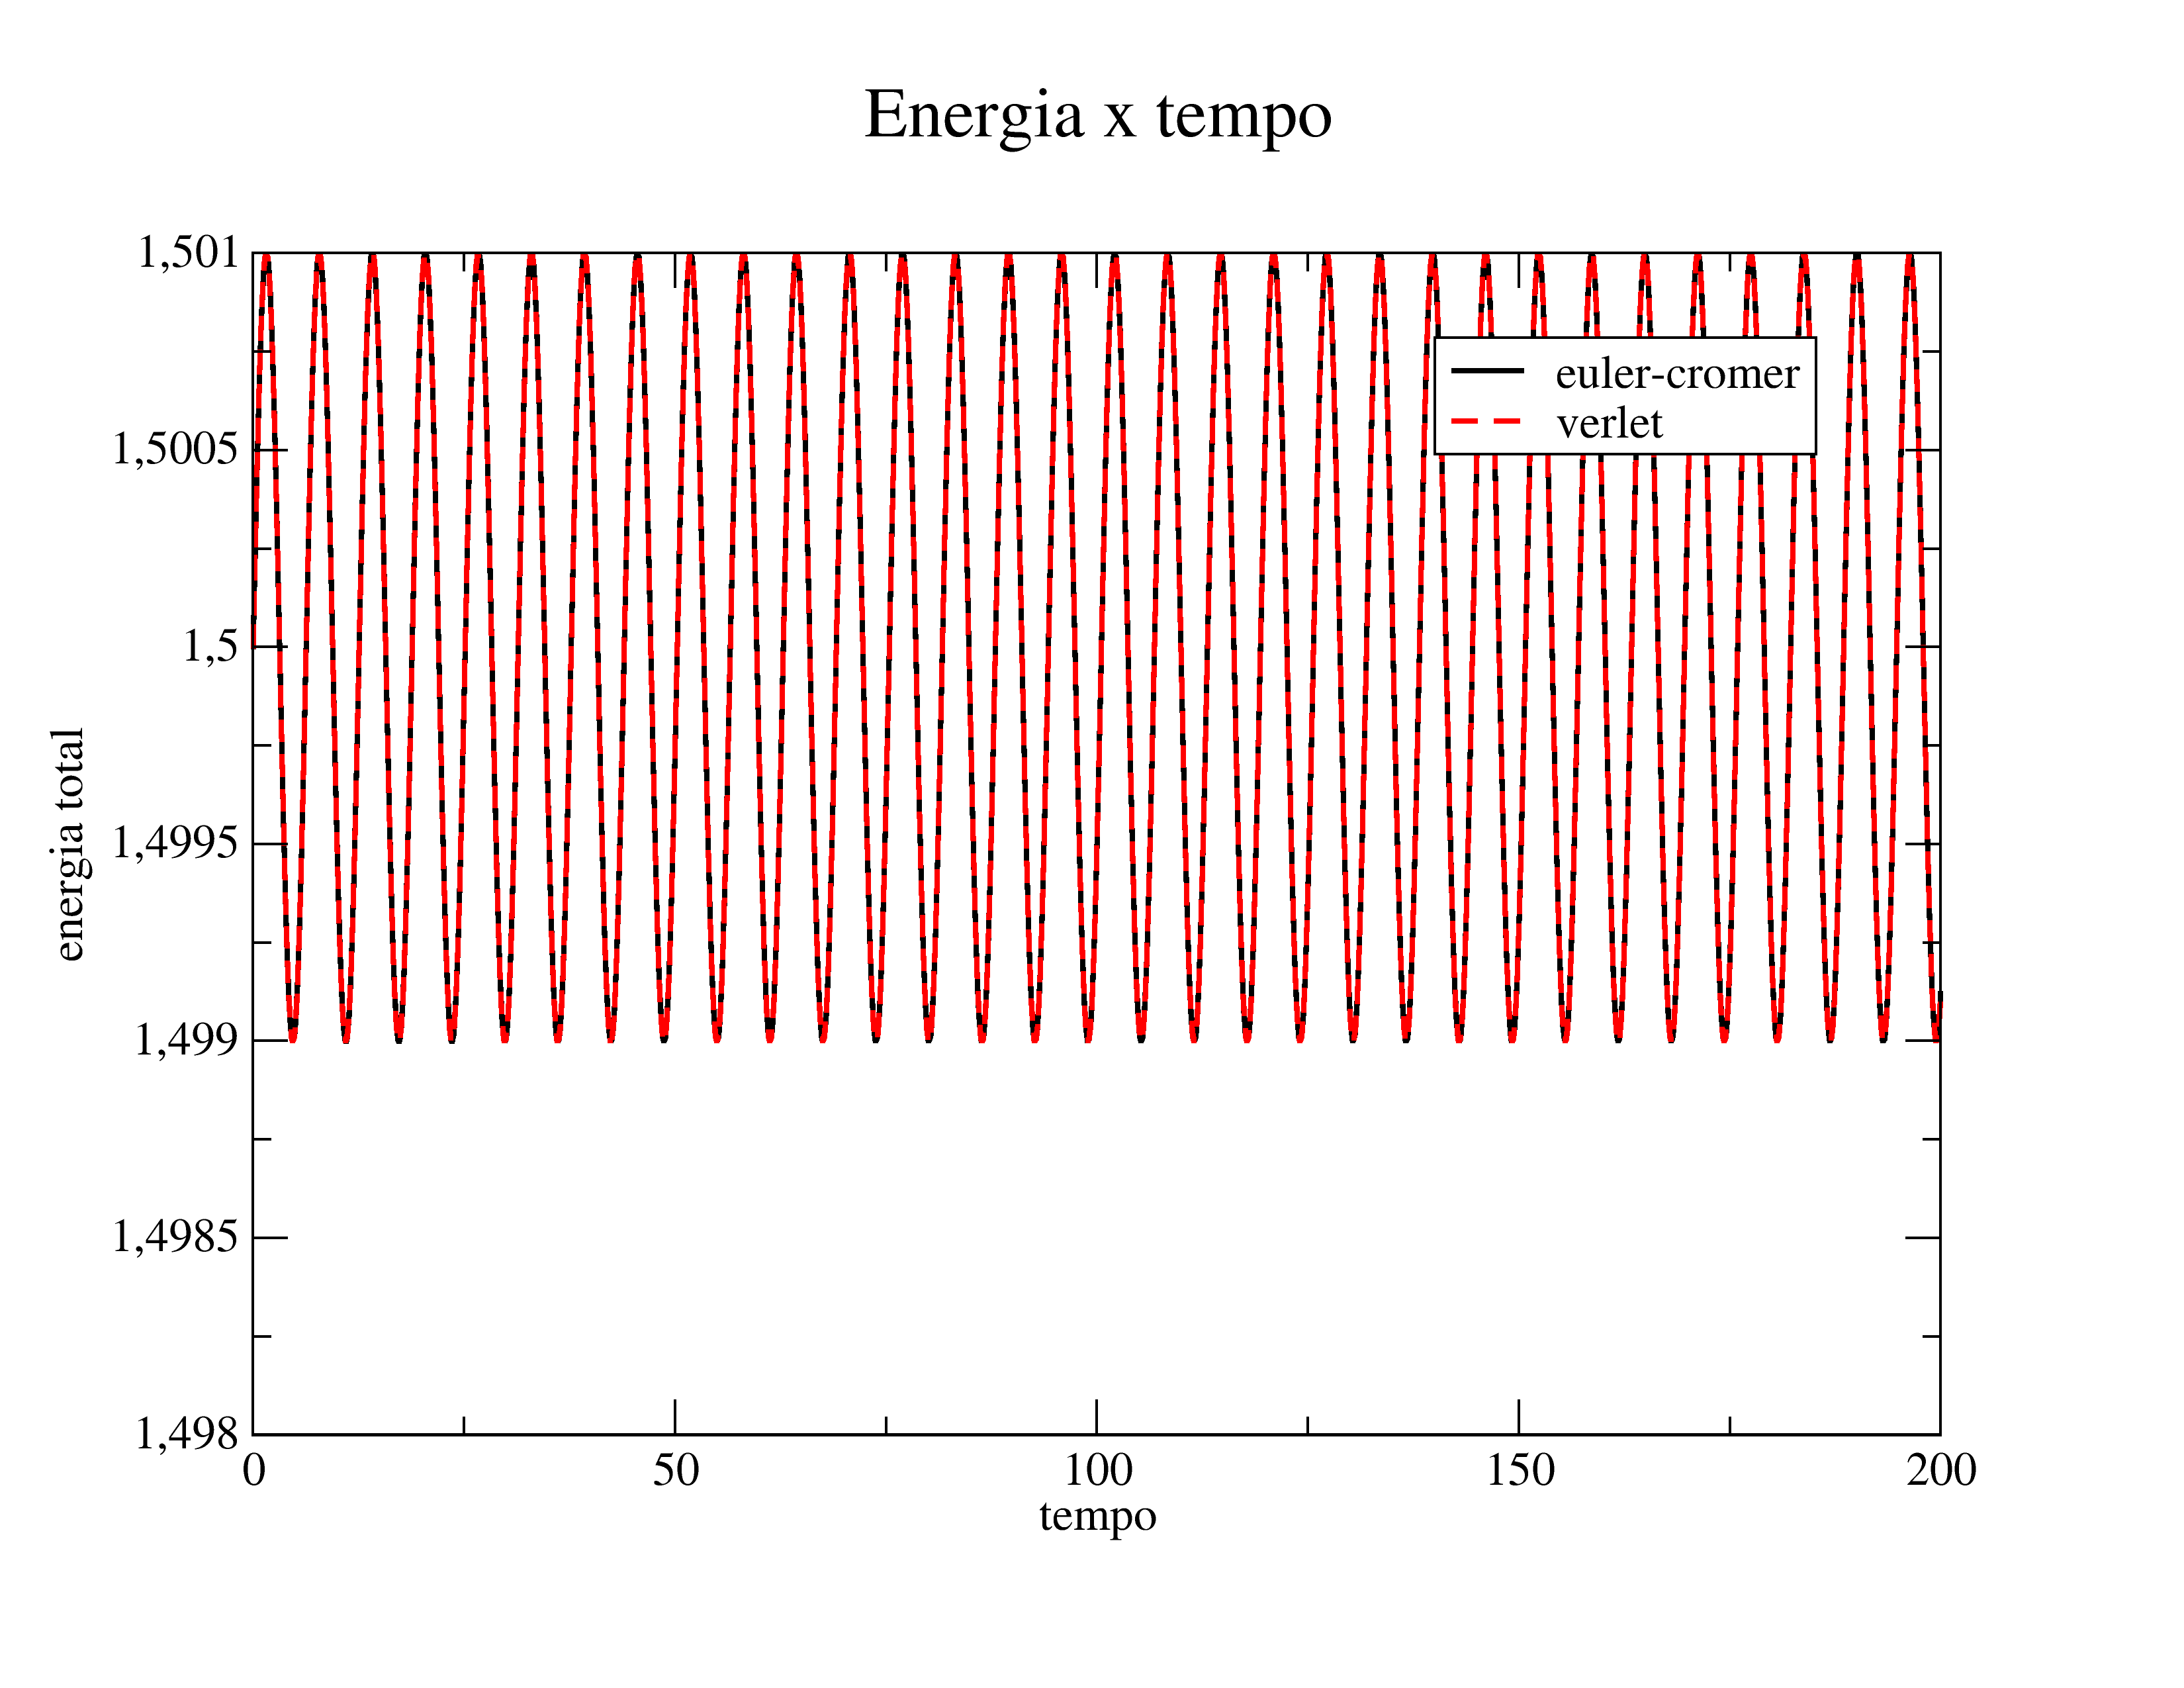
\includegraphics[width=\linewidth]{../tarefa-1d/energia.png}
\caption{Gráfico da energia adimensional}
\end{figure}

Percebemos que a energia vai variando bem pouco ao longo do tempo, mas permanece ao redor de $1.5$, o que é de se esperar pois estamos simulando a órbita da Terra, onde $\epsilon$ de fato vale $1.5$. Algo notável é que não percebemos nenhuma diferença entre o método de Euler-Cromer e o de Verlet nessa simulação, como podemos ver no gráfico.

\section{Tarefa 2}

\subsection{a}
Aqui vamos nos limitar a uma análise da órbita de Marte, cuja excentricidade já é conhecida. Temos dois programas, um para as primeiras duas leis e outro para a terceira lei. Seguem os ditos cujos:

\begin{minted}[
	mathescape,
	linenos,
	fontsize=\footnotesize,
	framesep=2mm,
	breaklines]
	{fortranfixed}
         implicit real*8 (a-h, o-z)
         real*8 p_ec(10000000,2)
         real*8 v_ec(10000000,2)
         real*8 p_verlet(10000000,2)
         real*8 v_verlet(10000000,2)

         pi = 4.d0*datan2(1.d0,1.d0)

         tau_total = 10d0
         dtau = 1d-4
         iteracoes = int(tau_total/dtau)
         a = 1d0
         a_marte = 1.662d0*a
         v_marte = 0.739d0

         open(file='orbita.dat', unit=1)
         open(file='1alei.dat',unit=2)
         open(file='2alei.dat', unit=3)

         p_ec(1,1) = 0d0
         p_ec(1,2) = a
         v_ec(1,1) = v_marte
         v_ec(1,2) = 0d0

         p_verlet(1,1) = p_ec(1,1)
         p_verlet(1,2) = p_ec(1,2)

         ymin = 10000d0
         ymax = 0d0

         ! para verificar se a órbita é elíptica, vamos descobrir qual é o y máximo e o y mínimo
         ! esse segundo será a distância do foco do sol, a um dos cantos da elipse
         ! o primeiro, subtraido pelo segundo, será a distância da origem até o segundo foco
         ! tendo isso, podemos verificar a 1a lei de kepler

         do i=2,iteracoes
            tempo = dble(i)*dtau
            p3 = pcubo(p_ec(i-1,1), p_ec(i-1,2))

            !verlet
            if (i.eq.2) then
               ! pular verlet, usar os valores de euler-cromer
               v_ec(i,1) = v_ec(i-1,1) - (p_ec(i-1,1)/p3)*dtau
               v_ec(i,2) = v_ec(i-1,2) - (p_ec(i-1,2)/p3)*dtau

               p_ec(i,1) = p_ec(i-1,1) + v_ec(i,1)*dtau
               p_ec(i,2) = p_ec(i-1,2) + v_ec(i,2)*dtau

               p_verlet(i,1) = p_ec(i,1)
               p_verlet(i,2) = p_ec(i,2)
            else
               p3 = pcubo(p_verlet(i-1,1),p_verlet(i-1,2))

               p_verlet(i,1) = 2d0*p_verlet(i-1,1) - p_verlet(i-2,1)
     &          - (p_verlet(i-1,1)/p3)*(dtau**2)
               p_verlet(i,2) = 2d0*p_verlet(i-1,2) - p_verlet(i-2,2)
     &          - (p_verlet(i-1,2)/p3)*(dtau**2)
            endif

            write(1,*)p_verlet(i,1), p_verlet(i,2)

            if (p_verlet(i,2).lt.ymin) then
               ymin = p_verlet(i,2)
            end if
            if (p_verlet(i,2).gt.ymax) then
               ymax = p_verlet(i,2)
            endif

            area = 0.5d0 * abs(p_verlet(i-1,1)*p_verlet(i,2)
     &      - p_verlet(i,1)*p_verlet(i-1,2))
            write(3,*)tempo, area


         end do


         foco = ymax - abs(ymin)
         write(*,*)ymin,ymax, foco

         ! agora verificar a 1a lei de kepler: calcular as distâncias em cada ponto a cada um dos focos
         do i=1,iteracoes
            tempo = dble(i)*dtau
            d1 = dsqrt(p_verlet(i,1)**2d0 + p_verlet(i,2)**2d0)
            d2 = dsqrt(p_verlet(i,1)**2d0 + (foco - p_verlet(i,2))**2d0)
            dist = d1+d2
            write(2,*)tempo,dist
         end do

         ! agora calcular as velocidades em Verlet
         ! vamos usar a derivdada simétrica de 5 pontos
         !do i=3,iteracoes-2
            ! começamos do 3 pq precisamos ter i-2 e i-1 válidos
         !   v_verlet(i,1) = (p_verlet(i-2,1) - 8d0*p_verlet(i-1,1)
     &   !    + 8d0*p_verlet(i+1,1) - p_verlet(i+2,1)) / (12d0*dtau)
         !   v_verlet(i,2) = (p_verlet(i-2,2) - 8d0*p_verlet(i-1,2)
     &   !    + 8d0*p_verlet(i+1,2) - p_verlet(i+2,2)) / (12d0*dtau)

          !  write(4,*)v_verlet(i,1), v_verlet(i,2)
         !end do


         end

         function pcubo(px,py)
            real*8 px, py, pcubo
            pcubo = (px**2d0 + py**2d0)**(3d0/2d0)
         end function

\end{minted}

\begin{minted}[
	mathescape,
	linenos,
	fontsize=\footnotesize,
	framesep=2mm,
	breaklines]
	{fortranfixed}
         implicit real*8 (a-h, o-z)
         real*8 p_ec(10000000,2)
         real*8 v_ec(10000000,2)
         real*8 p_verlet(10000000,2)
         real*8 v_verlet(10000000,2)

         pi = 4.d0*datan2(1.d0,1.d0)

         tau_total = 10d0
         dtau = 1d-5

         a = 1d0

         p_ec(1,1) = 0d0
         p_ec(1,2) = a
         v_ec(1,1) = 1d0/dsqrt(a)
         v_ec(1,2) = 0d0

         p_verlet(1,1) = p_ec(1,1)
         p_verlet(1,2) = p_ec(1,2)

         open(file='3alei.dat',unit=1)

         ! para verificar a 3a lei, vamos usar um exemplo simplificado para órbitas circulares
         ! e ir iterando em planetas imaginários até 5ua de raio

         do ip=1,10
            a = 0.5d0*dble(ip)
            p_ec(1,1) = a
            p_ec(1,2) = 0d0
            v_ec(1,1) = 0d0
            v_ec(1,2) = 1d0/dsqrt(a)

            p_verlet(1,1) = a
            p_verlet(1,2) = 0d0

            ! calcular periodo
            tau_total = 20d0*a
            iteracoes = int(tau_total/dtau)

            tempo_periodo = 0d0

         do i=2,iteracoes
            tempo = dble(i)*dtau
            p3 = pcubo(p_ec(i-1,1), p_ec(i-1,2))

            !verlet
            if (i.eq.2) then
               ! pular verlet, usar os valores de euler-cromer
               v_ec(i,1) = v_ec(i-1,1) - (p_ec(i-1,1)/p3)*dtau
               v_ec(i,2) = v_ec(i-1,2) - (p_ec(i-1,2)/p3)*dtau

               p_ec(i,1) = p_ec(i-1,1) + v_ec(i,1)*dtau
               p_ec(i,2) = p_ec(i-1,2) + v_ec(i,2)*dtau

               p_verlet(i,1) = p_ec(i,1)
               p_verlet(i,2) = p_ec(i,2)
            else
               p3 = pcubo(p_verlet(i-1,1),p_verlet(i-1,2))

               p_verlet(i,1) = 2d0*p_verlet(i-1,1) - p_verlet(i-2,1)
     &          - (p_verlet(i-1,1)/p3)*(dtau**2)
               p_verlet(i,2) = 2d0*p_verlet(i-1,2) - p_verlet(i-2,2)
     &          - (p_verlet(i-1,2)/p3)*(dtau**2)
            endif

            ! verificar se já deu 1 período
            if (tempo.gt.1d0)then
            if ((abs(p_verlet(1,1)-p_verlet(i,1)).lt.1d-3)
     &      .and.(abs(p_verlet(1,2)-p_verlet(i,2)).lt.1d-3)) then
               tempo_periodo = tempo
               goto 10
            endif
            endif
         end do

10       continue
         if (tempo_periodo.eq.0d0)then
            write(*,*)"Erro: nao achamos periodo p/",ip
         else
            write(*,*)"periodo p/",ip,tempo_periodo

            write(1,*)(a**3d0),(tempo_periodo**2d0)
         endif

         end do

         ! agora calcular as velocidades em Verlet
         ! vamos usar a derivdada simétrica de 5 pontos
         !do i=3,iteracoes-2
            ! começamos do 3 pq precisamos ter i-2 e i-1 válidos
         !   v_verlet(i,1) = (p_verlet(i-2,1) - 8d0*p_verlet(i-1,1)
     &   !    + 8d0*p_verlet(i+1,1) - p_verlet(i+2,1)) / (12d0*dtau)
         !   v_verlet(i,2) = (p_verlet(i-2,2) - 8d0*p_verlet(i-1,2)
     &   !    + 8d0*p_verlet(i+1,2) - p_verlet(i+2,2)) / (12d0*dtau)

          !  write(4,*)v_verlet(i,1), v_verlet(i,2)
         !end do


         end

         function pcubo(px,py)
            real*8 px, py, pcubo
            pcubo = (px**2d0 + py**2d0)**(3d0/2d0)
         end function

\end{minted}

Rodando o primeiro programa e graficando os resultados, obtemos:

\begin{figure}[H]
\centering
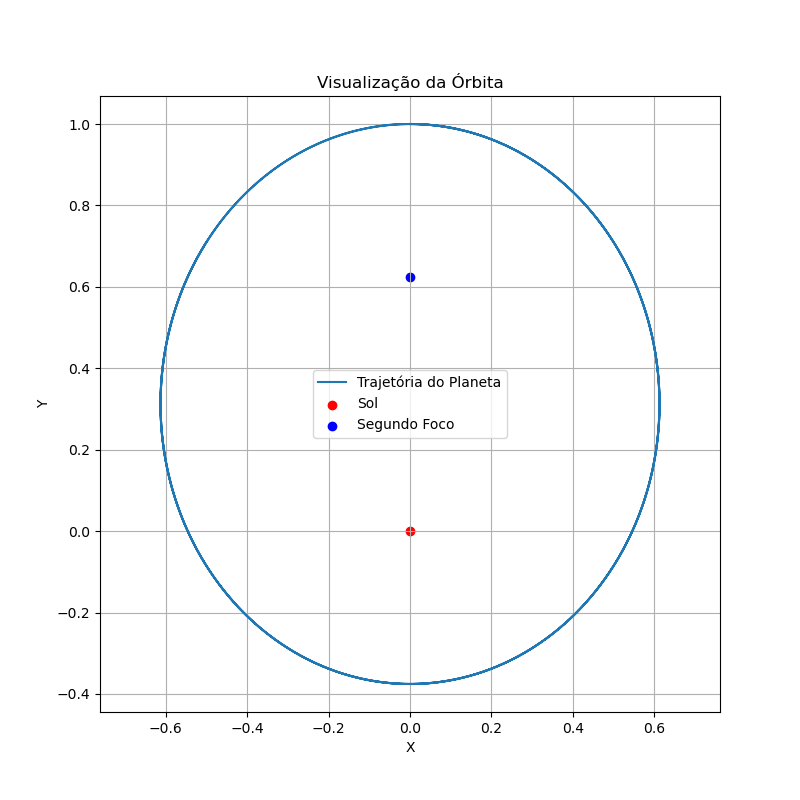
\includegraphics[width=\linewidth]{../tarefa-2a/orbita.png}
\caption{Gráfico da órbita de Marte simulada}
\end{figure}

Para descobrir a posição do 2o foco no nosso programa, basta apenas descobrir qual é a posição de menor valor de $y$ - a distância desta posição à origem será igual à distância do ponto de maior $y$ ao segundo foco. Neste caso, para a órbita de Marte, temos que a posição do sol é $(0,0)$ (claro) e a do segundo foco é $0.624$.

Agora, podemos verificar a 1a lei de Kepler, utilizando esse foco hipotético e verificando se a distância ao sol e ao foco, somadas, são constantes ao longo do tempo.

\begin{figure}[H]
\centering
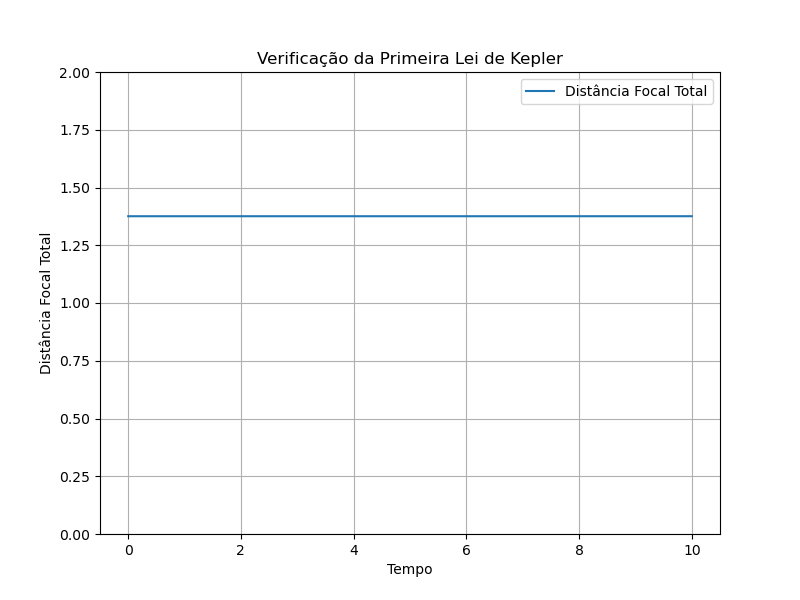
\includegraphics[width=\linewidth]{../tarefa-2a/1alei.png}
\caption{Gráfico da 1a lei de Kepler}
\end{figure}

De fato, a distância é constante ao longo do tempo! Portanto, a 1a lei está verificada.

Para vermos a 2a lei empregamos um procedimento similar, mas dessa vez calculando a área varrida em cada iteração do programa. Graficando, temos

\begin{figure}[H]
\centering
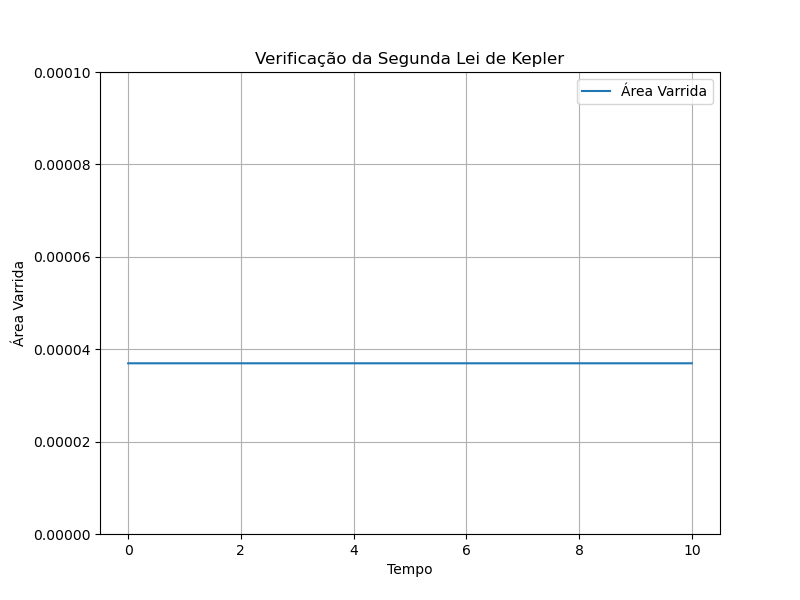
\includegraphics[width=\linewidth]{../tarefa-2a/2alei.png}
\caption{Gráfico da 2a lei de Kepler}
\end{figure}

Novamente, uma constante. Portanto, a 2a lei está verificada.

Para a 3a lei, simulamos diversos planetas e verificamos os seus períodos. Graficando isso, obtemos

\begin{figure}[H]
\centering
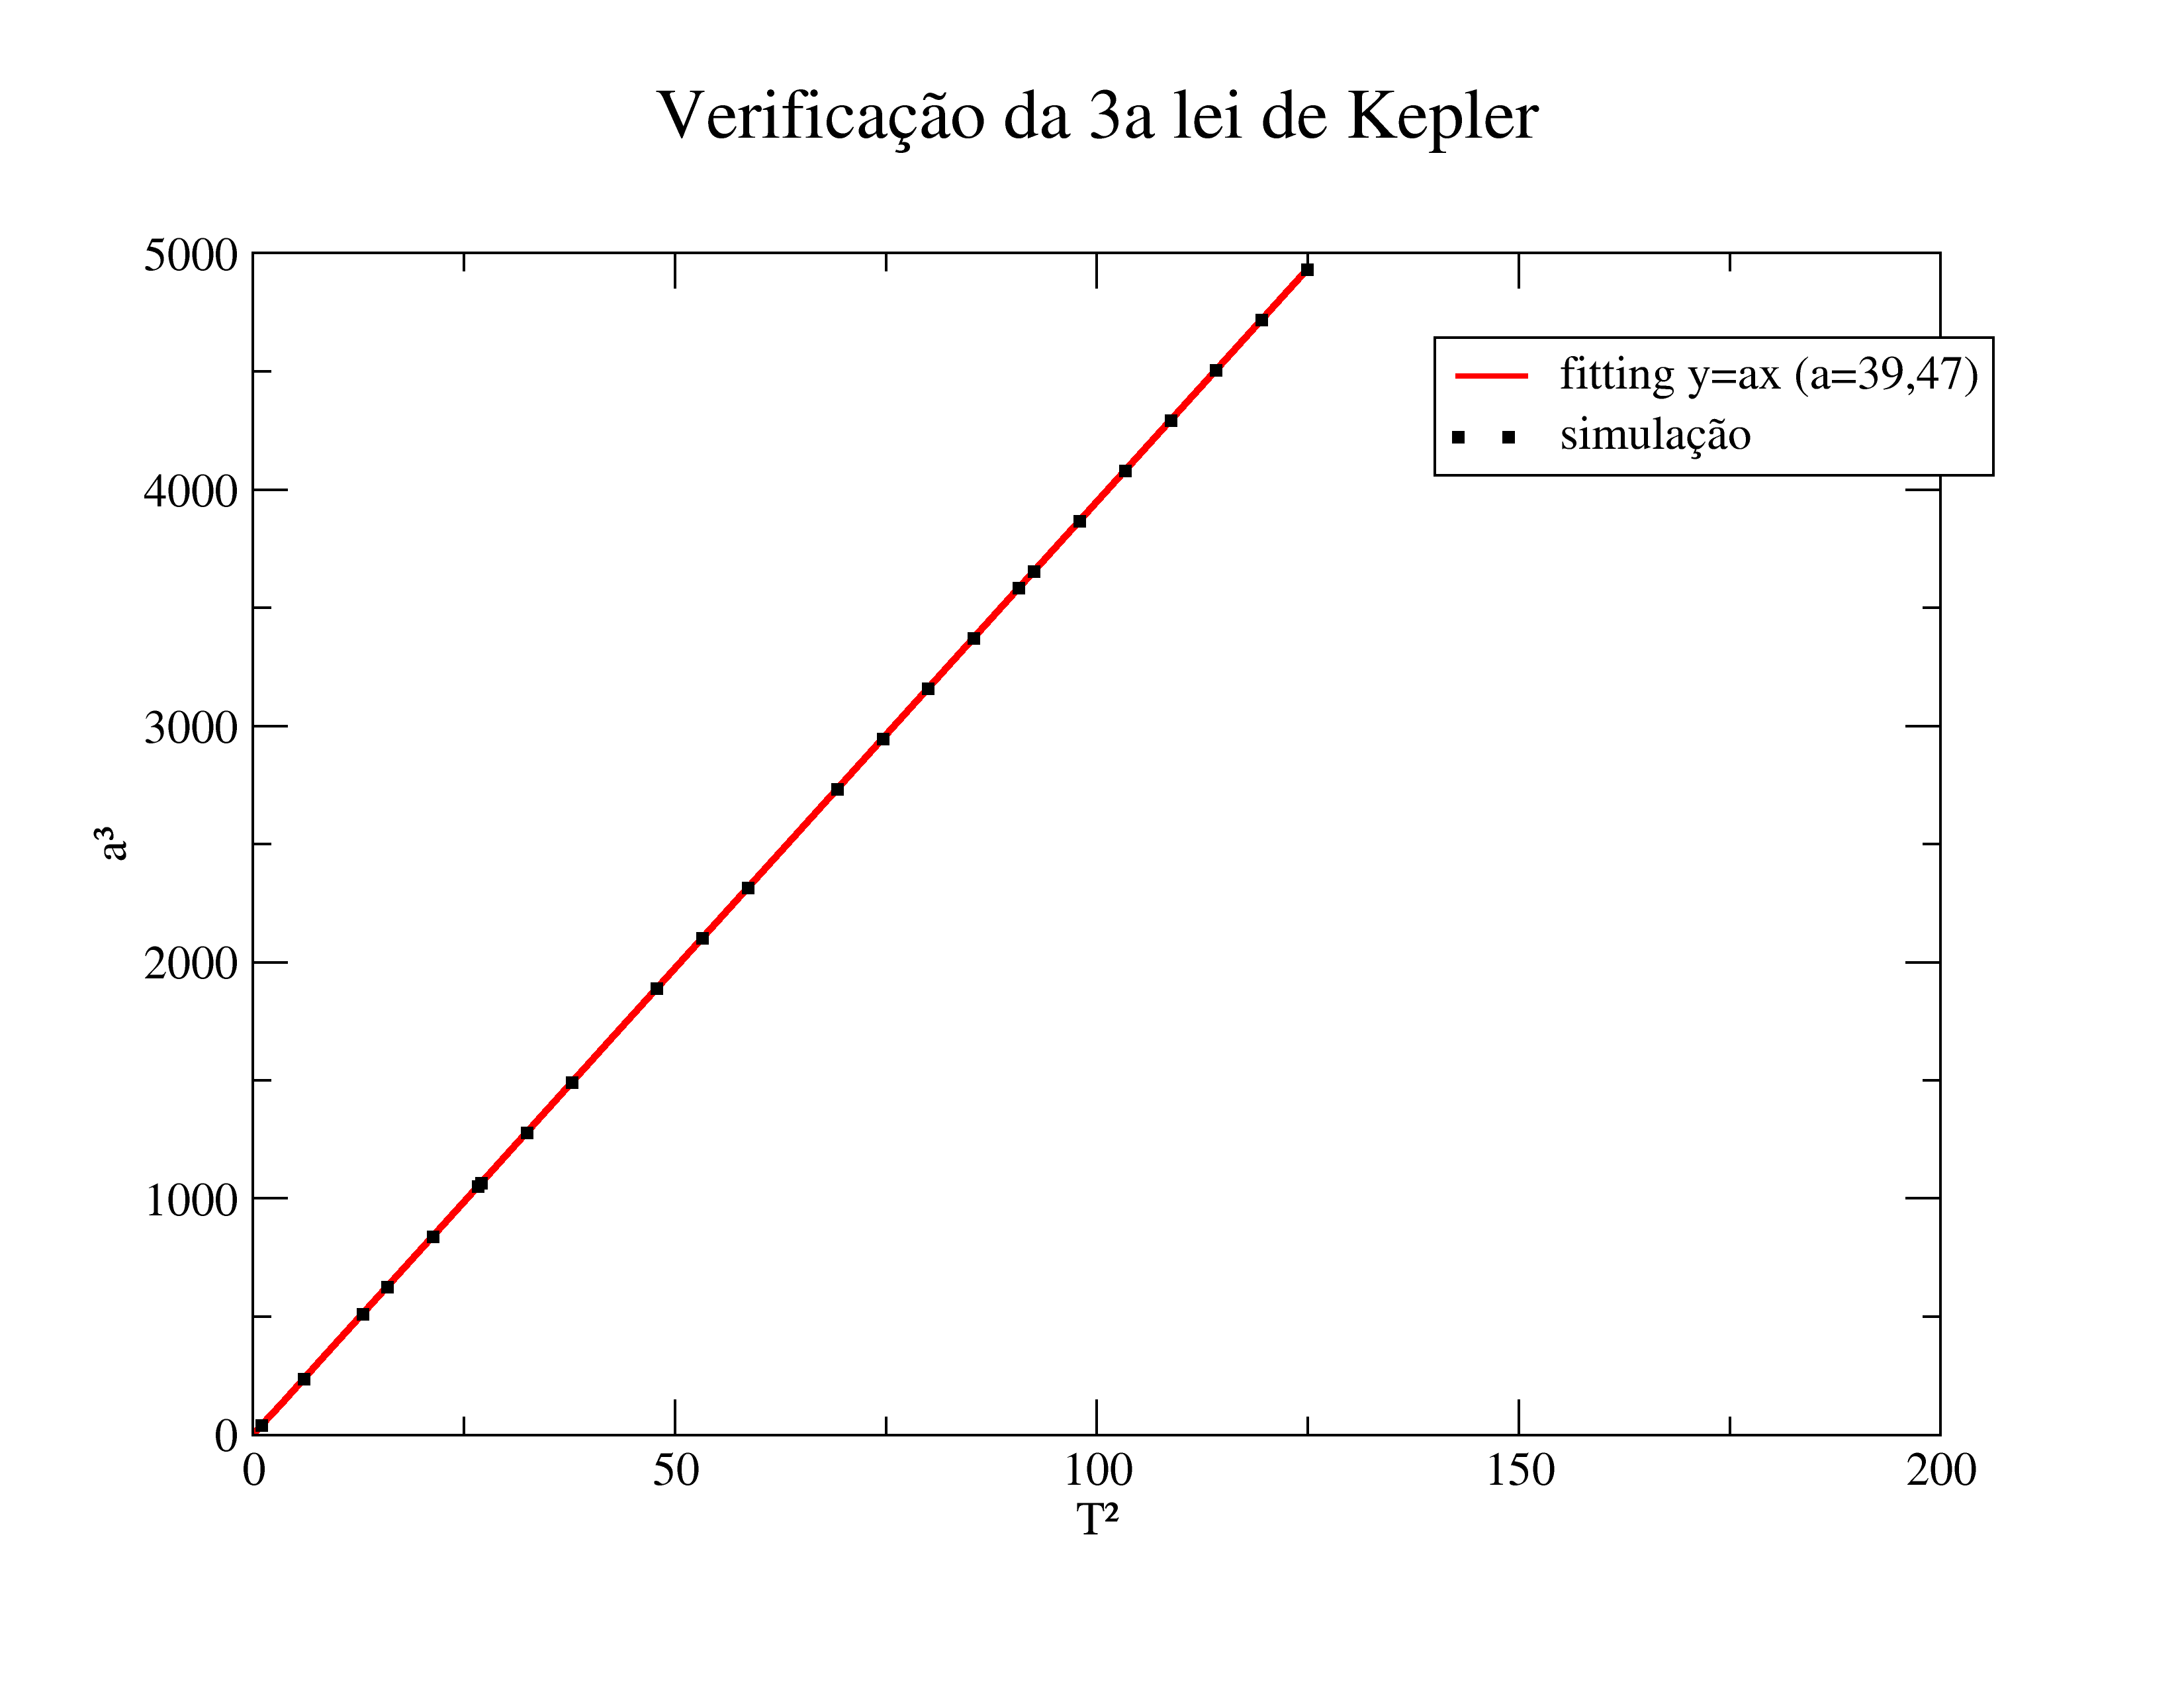
\includegraphics[width=\linewidth]{../tarefa-2a/grafico_3alei.png}
\caption{Gráfico da 3a lei de Kepler}
\end{figure}

Percebemos que a curva obtida é exatamente aquela que esperamos para $a^3 \propto T^2$, com a constante de proporcionalidade $39.47$, nas unidades adotadas. Portanto, verificamos também a 3a lei.

\section{Tarefa 3}
\subsection{a}

As equações de movimento são

\[ \vec{\ddot{\rho}}_t = \vec{a}_{ts} + \mu_j\vec{a}_{tj} \]
\[ \vec{\ddot{\rho}}_j = \vec{a}_{js} + \mu_t\vec{a}_{jt} \]

Para aplicar isso no método de Verlet basta apenas substituir na fórmula que já temos, isto é

\[ \vec{\rho}_{i+1} = 2\vec{\rho}_i - \vec{\rho}_{i-1} + \vec{\ddot{\rho}}_i(\Delta \tau)^2 \]

Nosso programa utiliza subrotinas para atualizar as acelerações da terra e de jupiter a cada iteração. Segue o programa:

\begin{minted}[
	mathescape,
	linenos,
	fontsize=\footnotesize,
	framesep=2mm,
	breaklines]
	{fortranfixed}
      implicit real*8 (a-h, o-z)
      real*8 p_t(100000000, 2)
      real*8 p_j(100000000, 2)
      real*8 at(2),aj(2)

      open(file='terra.dat',unit=1)
      open(file='jupiter.dat', unit=2)

      pi = 4.d0*datan2(1.d0,1.d0)

      tau_total = 2d0*pi*30d0 ! 30 anos
      dtau = 1d-3

      p_t(1,1) = 1d0
      p_t(1,2) = 0d0
      p_j(1,1) = 5.2d0
      p_j(1,2) = 0d0

      v_tx = 0d0
      v_ty = 1d0
      v_jx = 0d0
      v_jy = 1d0/dsqrt(5.2d0)

      iteracoes = tau_total/dtau

      iunidade = 10000

      ! fazer iterações ser divisível por iunidade (p ficar bonitinha a divisao no progresso)
      if (mod(iteracoes,iunidade).ne.0) then
         iteracoes = (iteracoes/iunidade + 1)*iunidade
      endif

      do i=2,iteracoes
         if (mod(i,iunidade).eq.0) then
            write(*,*)'progresso:',int((dble(i)/dble(iteracoes))*100)
         endif

         ! equações de movimento p/ terra e júpiter
         call acel_t(p_t(i-1,1),p_t(i-1,2),p_j(i-1,1),p_j(i-1,2), at)
         call acel_j(p_j(i-1,1),p_j(i-1,2),p_t(i-1,1),p_t(i-1,2), aj)

         if (i.eq.2) then
            ! usar euler-cromer

            ! terra
            v_tx = v_tx - at(1)*dtau
            v_ty = v_ty - at(2)*dtau
            p_t(i,1) = p_t(i-1,1) + v_tx*dtau
            p_t(i,2) = p_t(i-1,2) + v_ty*dtau

            ! jupiter
            v_jx = v_jx - aj(1)*dtau
            v_jy = v_jy - aj(2)*dtau
            p_j(i,1) = p_j(i-1,1) + v_jx*dtau
            p_j(i,2) = p_j(i-1,2) + v_jy*dtau

         else
            ! terra
            p_t(i,1) = 2d0*p_t(i-1,1) - p_t(i-2,1) +
     &      at(1)*(dtau**2d0)
            p_t(i,2) = 2d0*p_t(i-1,2) - p_t(i-2,2) +
     &      at(2)*(dtau**2d0)

            !jupiter
            p_j(i,1) = 2d0*p_j(i-1,1) - p_j(i-2,1) +
     &      aj(1)*(dtau**2d0)
            p_j(i,2) = 2d0*p_j(i-1,2) - p_j(i-2,2) +
     &      aj(2)*(dtau**2d0)
            endif

         write(1,*)p_t(i,1),p_t(i,2)!, at
         write(2,*)p_j(i,1),p_j(i,2)

      end do

      end

      subroutine acel_t(px,py,pjx,pjy,at)
         ! modifica a aceleração da terra dados p_t e p_j
         real*8 px,py,pjx,pjy,atsx,atsy,mu_j,mu_t,atjx,atjy,p3
         real*8 at(2)

         mu_t = 1d0/(3.33d5)
         mu_j = 318d0/(3.33d5)

         p3 = (px**2d0 + py**2d0)**1.5d0
         p3j = ( (px-pjx)**2d0 + (py-pjy)**2d0 )**1.5d0

         atsx = -px/p3
         atsy = -py/p3

         atjx = -(px-pjx)/p3j
         atjy = -(py-pjy)/p3j

         at(1) = atsx + mu_j*atjx
         at(2) = atsy + mu_j*atjy

      end subroutine

      subroutine acel_j(px,py,ptx,pty,aj)
         ! modifica a aceleração de jupiter dados p_t e p_j
         real*8 px,py,ptx,pty,ajsx,ajsy,mu_j,mu_t,ajtx,ajty,p3
         real*8 aj(2)

         mu_t = 1d0/(3.33d5)
         mu_j = 318d0/(3.33d5)

         p3 = (px**2d0 + py**2d0)**1.5d0
         p3t = ( (px-ptx)**2d0 + (py-pty)**2d0 )**1.5d0

         ajsx = -px/p3
         ajsy = -py/p3

         ajtx = -(px-ptx)/p3t
         ajty = -(py-pty)/p3t

         aj(1) = ajsx + mu_j*ajtx
         aj(2) = ajsy + mu_j*ajty

      end subroutine
\end{minted}

\subsection{b}
Aqui utilizaremos o menor $\Delta \tau$ de que precisaríamos de acordo com os resultados da tarefa 1c, que, no caso, é de $10^{-3}$.

Graficando a órbita da Terra durante 30 anos, temos

\begin{figure}[H]
\centering
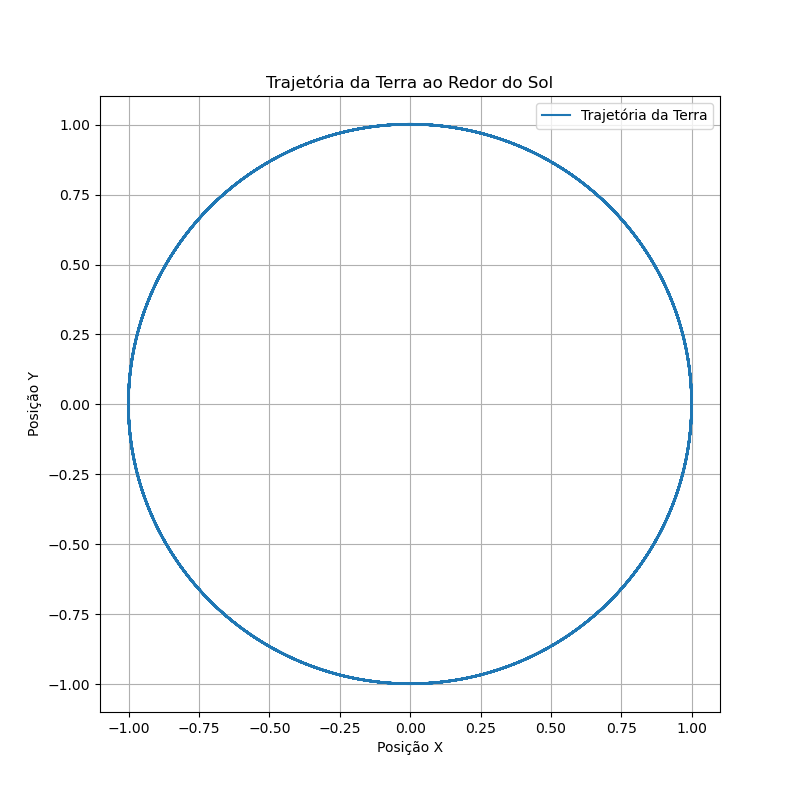
\includegraphics[width=\linewidth]{../tarefa-3/orbita1.png}
\caption{Órbita de terra com Júpiter no sistema}
\end{figure}

Percebemos que, se dermos um grande zoom, a órbita está variando ao longo do tempo:

\begin{figure}[H]
\centering
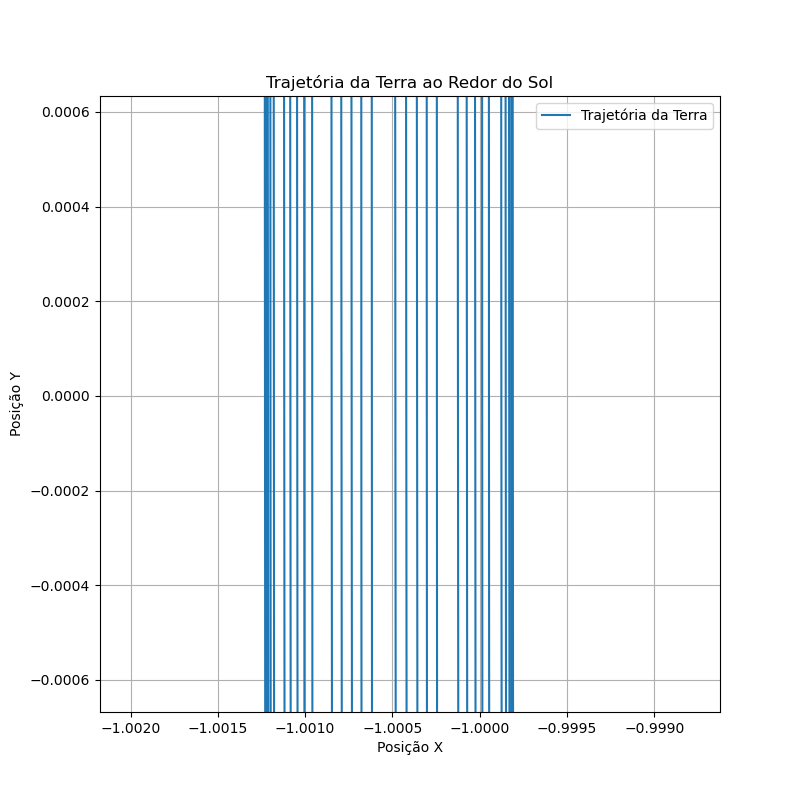
\includegraphics[width=\linewidth]{../tarefa-3/orbita2.png}
\caption{Órbita de terra com Júpiter no sistema - com zoom}
\end{figure}

Isto ocorre devido à atração gravitacional de Júpiter.

\subsection{c}

Multiplicando a massa de Júpiter por 100, achei legal fazer uma animação do resultado, que pode ser vista nesse link:

\url{https://youtu.be/CYUy6Q7UrLI}

Sem animação, temos os seguintes dois gráficos:

\begin{figure}[H]
\centering
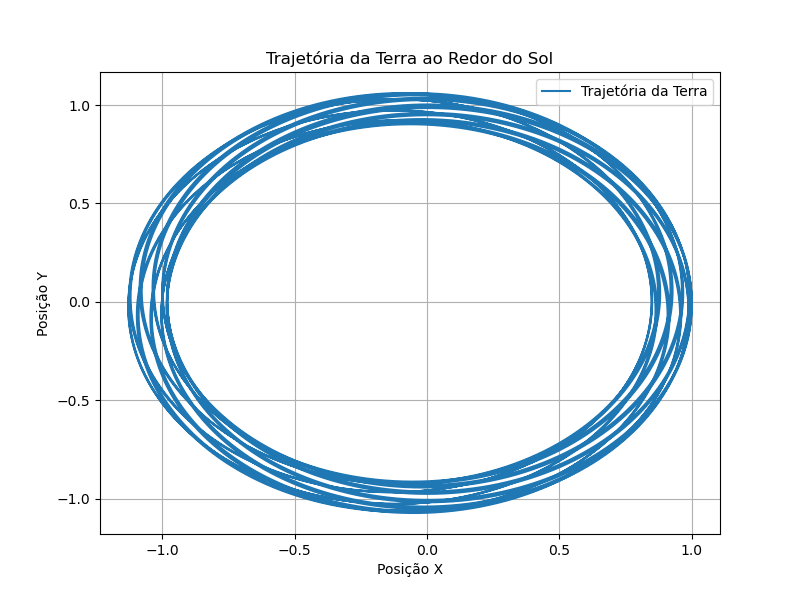
\includegraphics[width=\linewidth]{../tarefa-3/terra.png}
\caption{Órbita de terra com júpiter 100x mais massivo}
\end{figure}

\begin{figure}[H]
\centering
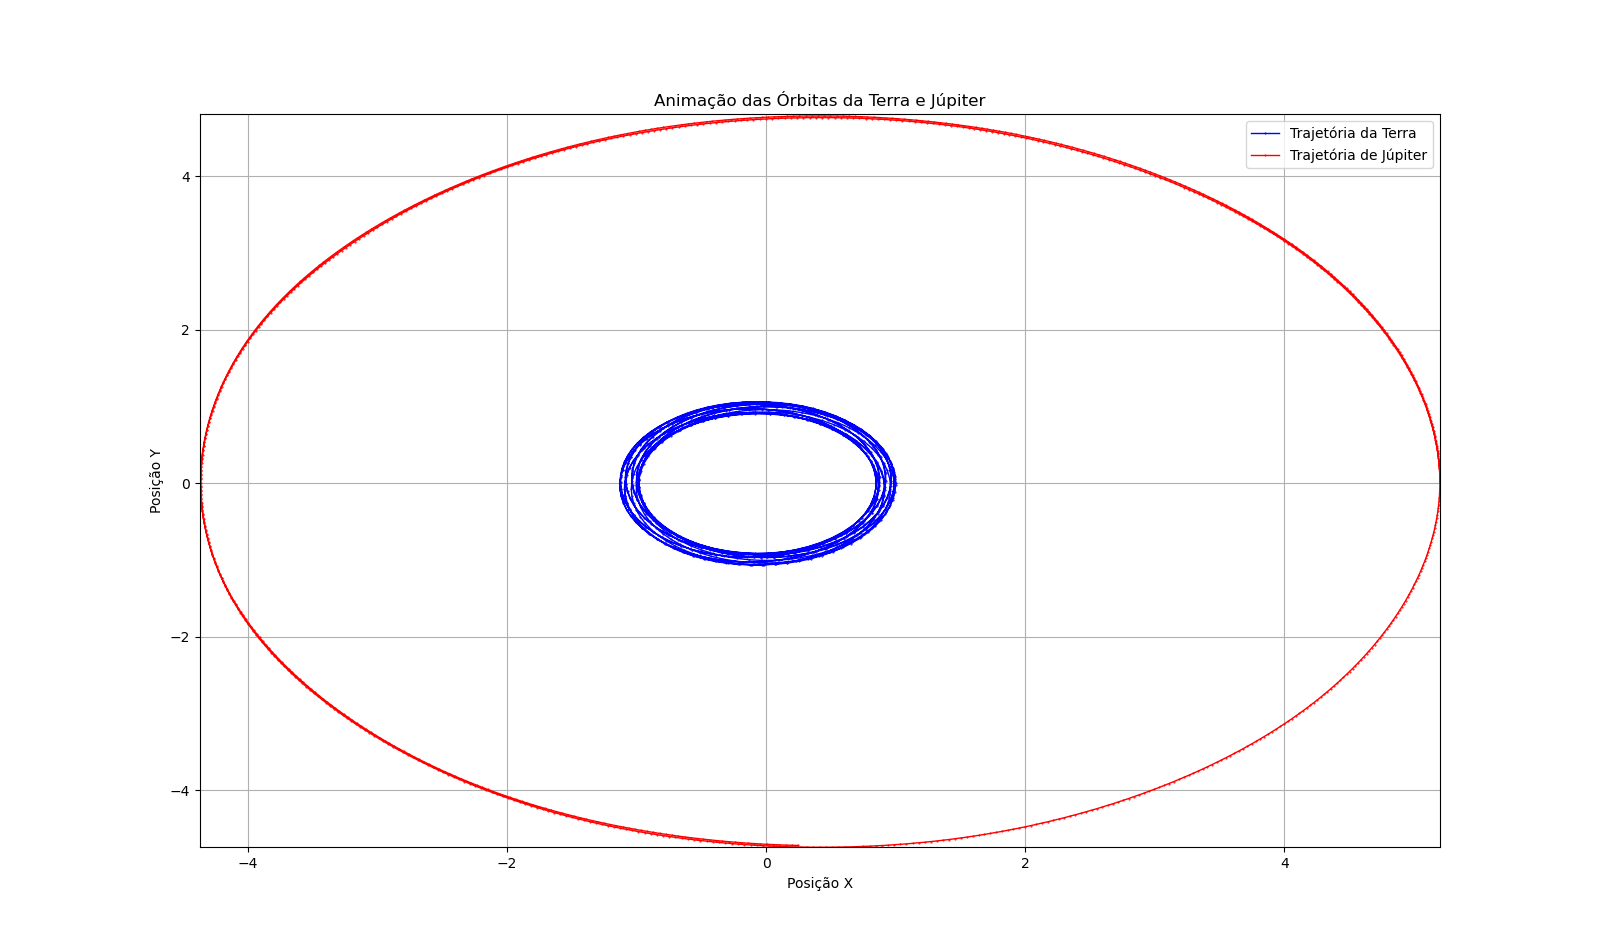
\includegraphics[width=\linewidth]{../tarefa-3/terrajupiter100.png}
\caption{Órbita de terra e de júpiter, com júpiter 100x mais massivo}
\end{figure}

Percebemos que a órbita da terra vai oscilando dependendo de onde fica a posição de Júpiter, o que faz com que ela não tenha uma "órbita" específica estável. Porém, parece que ela não sai muito da área onde ela está, apenas fica oscilando em sua órbita. Isso pode ser visualizado melhor na animação.

Agora, multiplicamos a massa de Júpiter por 1000 ao invés de 100, e temos um resultado muito interessante:

\url{https://www.youtube.com/watch?v=CA9KG9WjM50}

O sistema é caótico! Agora não temos mais sistema solar, mas mesmo assim a animação é muito bonita e legal de assistir.

\end{document}